\documentclass[12pt]{report}
\usepackage[utf8x]{inputenc}
\usepackage[T1]{fontenc}
\usepackage[francais]{babel}
\usepackage{graphicx}
\usepackage{amsfonts}
\usepackage{hyperref}
\usepackage{fnpct}
\usepackage{array}
\usepackage{titlesec}
\usepackage{amssymb}
\usepackage[normalem]{ulem}
\useunder{\uline}{\ul}{}

% --------------INTEGRATION CODE JAVA----------
\usepackage{listings}
\lstset{
language=Java,
basicstyle=\normalsize, % ou ça==> basicstyle=\scriptsize,
upquote=true,
aboveskip={1.5\baselineskip},
columns=fullflexible,
showstringspaces=false,
extendedchars=true,
breaklines=true,
showtabs=false,
showspaces=false,
showstringspaces=false,
identifierstyle=\ttfamily,
keywordstyle=\color[rgb]{0,0,1},
commentstyle=\color[rgb]{0.133,0.545,0.133},
stringstyle=\color[rgb]{0.627,0.126,0.941},
}
%-------------------------------------------------------

\usepackage{diagbox}
\usepackage{geometry}
\geometry{hmargin=2.5cm,vmargin=1.5cm}

\titlespacing*{\subsection}{30pt}{15pt}{10pt}
\titlespacing*{\subsubsection}{0pt}{15pt}{5pt}

% Packages graphiques
\usepackage{caption} 
\captionsetup{justification=centering}
\usepackage{tikz}
\usepackage{mathtools}
\usepackage{amsmath}
\usepackage{pgfplots}
\usepackage{pdfpages}
\usepackage{adjustbox}
\usetikzlibrary{plotmarks}
\pgfplotsset{compat=1.8}

\renewcommand{\thesubsubsection}{}
\renewcommand{\theparagraph}{}
\usepackage{blindtext}
\usepackage{chngcntr}
\usepackage[nottoc, notlof, notlot]{tocbibind}
\counterwithin*{section}{chapter}

\title{Guidage d'une personne malvoyante via une application GPS sur smartphone}
\author{Guitard \and Ouaraqua Dantchiawa \and Marcy \and Berthelot}
\date{\today}
\begin{document}
\setcounter{secnumdepth}{3}
\begin{titlepage}

\newcommand{\HRule}{\rule{\linewidth}{0.5mm}} 

\center 

\textsc{\LARGE Université de Bordeaux}\\[1.5cm] 
\textsc{\Large Département Informatique}\\[0.5cm] 
\textsc{\large Projet de Programmation}\\[0.5cm] 

%----------------------------------------------------------------------------------------
%	TITRE
%----------------------------------------------------------------------------------------

\HRule \\[0.5cm]
{ \LARGE \bfseries Guidage d’une personne malvoyante via une application GPS sur smartphone}\\[0.5cm]
\HRule \\[1.5cm]
 
%----------------------------------------------------------------------------------------
%	AUTEURS
%----------------------------------------------------------------------------------------

\begin{minipage}{0.4\textwidth}
\begin{flushleft} \large
\emph{Auteurs:}\\
Alan \textsc{Guitard}\\
Mohamed Ouaraqua \textsc{ Dantchiawa}\\
Nicolas \textsc{Marcy}\\
Florian \textsc{Berthelot}\\

\end{flushleft}
\end{minipage}
~
\begin{minipage}{0.4\textwidth}
\begin{flushright} \large
\emph{Encadrant:} \\
Matthieu \textsc{Raffinot}\\
\emph{Client:}\\
Serge \textsc{Chaumette} 
\end{flushright}
\end{minipage}\\[2cm]



%----------------------------------------------------------------------------------------
%	DATE 
%----------------------------------------------------------------------------------------

{\large \today}\\[1.5cm] % Date

%----------------------------------------------------------------------------------------
%	LOGO
%----------------------------------------------------------------------------------------


\includegraphics[height=80px]{Assets/logoUniversite.jpg}\\[1cm] % Logo université
 
%----------------------------------------------------------------------------------------

\vfill 

\end{titlepage}

\tableofcontents

\newpage

\chapter*{Remerciements}
\addcontentsline{toc}{chapter}{Remerciements}

Nous tenons à remercier toutes les personnes qui ont contribué à la réalisation de ce projet, à savoir \textbf{Monsieur Philippe Narbel}, responsable du cours intitulé \textit{Projet de programmation} et du \textit{Master Génie Logiciel}, qui nous a donné des conseils par ses cours. Et de vive voix, \textbf{Monsieur Mathieu Raffinot}, notre chargé de TD, qui nous prodigué ses conseils dans le développement, nous a motivé au début du projet lorsqu'on avait du mal à commencer et a défendu notre projet auprès des personnes qui jugent notre travail. Également, nous remercions \textbf{Monsieur Serge Chaumette} qui nous a proposé le sujet du projet et nous a consacré le peu de temps qu'il avait pour nous expliquer ses attentes et pour nous prêter des téléphones du laboratoire du \textit{LaBRI} pour un meilleur confort de développement.
\begin{abstract}
Ce projet a été réalisé sous la direction de Matthieu Raffinot, chercheur CNRS, dans le cadre du Master 1 Génie logiciel lié au cours de Projet de Programmation, dirigé par Philippe Narbel, maître de conférence. Le projet a pour but pédagogique de nous initier au génie Logiciel, et plus précisément à la gestion et l'organisation d'un projet en équipe.\\

Le sujet proposé par le client est de permettre à une personne malvoyante de pouvoir utiliser une application \textit{Android} de guidage par GPS afin de se rendre à une destination, de préférence à pied. L'application doit donc s'adapter à la vue défaillante de l'utilisateur et ainsi proposer une interface ergonomique. L'utilisateur aura la possibilité d'utiliser deux modes d'utilisation. Le premier mode sera utilisable avec deux téléphones qui symboliseront chacun une direction, le téléphone de gauche vibrera lorsque l'utilisateur devra tourner à gauche et le téléphone de droite vibrera lorsque l'utilisateur devra tourner à droite. Le second mode sera proposé si l'utilisateur ne possède qu'un seul téléphone fonctionnel qui vibrera une fois pour la direction de gauche, et deux fois pour la direction de droite.\\

Pour ce faire, on a donc eu besoin d'exploiter les technologies natives du téléphone : le GPS, les capteurs de navigation inertielle, le vibreur et le \textit{BlueTooth}. L'application sera développée sur un téléphone mobile sous système \textit{Android}, en utilisant le langage de programmation Java, le kit de développement \textit{Android} et l'API \textit{Google} pour la navigation.\\

Il est à noter que l'utilisation de cette application ne remplace pas les moyens habituelles que l'utilisateur utilise pour se déplacer seul (canne, chien d'aveugle, ...). A l'instar d'un GPS classique qui n'exempte pas les conducteurs du respect du code de la route, l'application est uniquement un guide.
\end{abstract}
\chapter*{Introduction}
\addcontentsline{toc}{chapter}{Introduction}
Lorsqu'une personne malvoyante compte se rendre à une destination dans une ville, des applications GPS lui sont disponibles grâce à une option de commande vocale, qui lui indique la route à suivre. Le problème que l'on peut constater avec cette voix qui lui sert de guide est que, pour l'entendre en pleine rue, l'utilisateur se voit obligé de brancher des écouteurs à l'appareil s'il ne veut pas mettre de haut-parleurs pour rester discret. Il serait donc utile à ces personnes, dont les oreilles sont pour eux le principal organe qui leur permettent de se situer dans l'espace, d'avoir une fonctionnalité qui leur permettrait une plus grande discrétion.\\

Le projet aura donc pour but de fournir à l'utilisateur une fonction de guidage par la vibration des téléphones, en donnant à l'utilisateur la possibilité de lier deux téléphones par une connexion \textit{BlueTooth} afin que le téléphone principal soit dédié à vibrer quand l'utilisateur doit tourner à gauche, et l'autre à droite, ou inversement.\\

Il est important de noter que le projet a pour but principal de nous apprendre à travailler en groupe sur un projet assez conséquent. Afin de gérer ce type de projet, une grande rigueur dans l'organisation est de mise.\\

La première étape était d'abord d'apprivoiser le fonctionnement de l'environnement mobile, de comprendre les concepts de la programmation sur système \textit{Android} et de mettre en place le dépôt SVN du projet sur le serveur \textit{Savane} du \textit{CREMI} afin d'assurer cette rigueur obligatoire pour les projets de cette échelle.\\

Dans une première partie, nous présenterons le contexte de développement et le cahier des charges du projet, qui comprend l'analyse des besoins, des schémas de scénarios et des diagrammes UML.
Dans un deuxième temps, nous détaillerons l'architecture du projet, le lien entre les différents modules du projet et leur évolution.
Ensuite, nous entamerons la question des tests, qu'ils soient unitaires ou d'intégration, et nous expliquerons le fonctionnement précis de l'application. Enfin, nous conclurons en détaillant à quel point en est le projet, les améliorations que l'on peut lui apporter et nous dresserons un bilan du cycle de développement que nous avons parcouru.
\chapter{Contexte et présentation du projet}

\section{Contexte et analyse de l'existant}

\subsection{Contexte}

\subsubsection{Choix des technologies utilisées}
Considérant l'émergence du smartphone ces dernières années et la plus grande accessibilité de \textit{Google} comparé à \textit{Apple} quant à ses mobiles et à ses kits de développement, l'application sera développée sur \textit{Android}. Pour la navigation, l'API \textit{Google} étant mise à disposition pour les développeurs et relativement facile à utiliser, elle s'est vite imposée comme choix d'implémentation. Enfin, l'IDE \textit{Android Studio}\footnote{\url{http://developer.android.com/sdk/index.html}}, supporté par \textit{Google}, a été choisi pour sa complémentarité avec le kit de développement \textit{Android} et ses nombreuses fonctionnalités.\\

\subsubsection{La société \emph{Google}} Filiale depuis 2005 de la société Alphabet en Californie, elle a été créé en 1998 par Larry Page et Sergueï Brin, les créateurs du moteur de recherche éponyme très connu. Elle est devenue au fil des années une des entreprises les plus importantes du Monde, étant celle la plus chèrement cotée en bourse avec une capitalisation boursière de 550 milliards de dollars.\newline
\textit{Google} s'est placé habilement auprès des développeurs par sa contribution à la technologie \underline{Open Source}, lui permettant non seulement de repérer les talents au cours d'événements tel que le \textit{Google Summer of Code}\footnote{\url{https://developers.google.com/open-source/gsoc/?csw=1}}, mais aussi de permettre à la communauté de développer en privé des logiciels sur leur plate-forme, et ainsi de contribuer à la vie de \textit{Google}.

\subsubsection{Le système d'exploitation \emph{Android}} C'est un système d'exploitation mobile basé sur le noyaux Linux, distribué en \underline{Open Source} sous licence Apache\cite{Apache} profitant des services système de base tels que la sécurité, la gestion mémoire ou la gestion de processus.

Le système est organisé en cinq couches: le noyau Linux, les bibliothèques logicielles (OpenGL, WebGL, SQLite,...), un environnement d'exécutions et bibliothèque pour la plate-forme Java, un kit de développement et enfin les applications standards comme un navigateur web, le carnet d'adresses ou l'application de messagerie et de téléphonie mobile.
\textit{Android} bénéficie d'une architecture en couche complète faisant de lui une plateforme riche, dédiée aux appareils mobiles. Depuis le 5 Octobre 2015, les téléphones sont maintenant vendues avec la version 6.0.1 d'\textit{Android}, aussi appelée \textit{Marshmallow}. 

\begin{center}
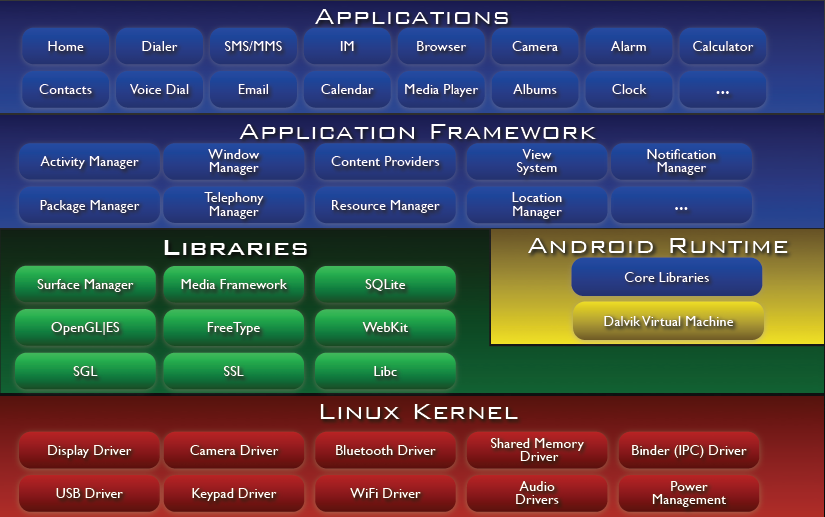
\includegraphics[height=300px]{Assets/androidArchi.png}
\begin{flushleft}
\hspace*{15pt}\hbox{\scriptsize Source:\thinspace{\scriptsize \itshape \url{http://www-igm.univ-mlv.fr/~dr/XPOSE2008/android/archi_comp.html}}}
\end{flushleft}
\captionof{figure}{Architecture Android}

\end{center}

\subsubsection{Fonctionnement d'une application}

Le développement d'une application \textit{Android} se produit au moyen d'un système de compilation automatique, \textit{Gradle} ou \textit{Maven}, qui permettent d'automatiser l'intégration des dépendances. Le langage Java est utilisé, accompagné de multiples extensions intégrées au SDK \textit{Android}, tel que la gestion des activités, leur contexte et l'interaction avec les composants de l'appareil. Le système \textit{Android} fonctionne avec une pile d'activités. Une activité qui se lance est placée en haut de la pile et peut très bien se faire "empiler" par d'autres activités (venant de la même application ou non). Lorsqu'une activité n'est pas au premier plan, elle est soit en pause, soit arrêtée. Ces \underline{activités}, qui composent une application, sont composées de \underline{vues} (éléments graphiques) comportant des \underline{widgets} (boutons, input, etc). L'agencement des éléments graphiques est effectué grâce à des vues spéciales, appelées \underline{layouts}.

\subsubsection{Fonctionnement d'une activité}

\begin{center}
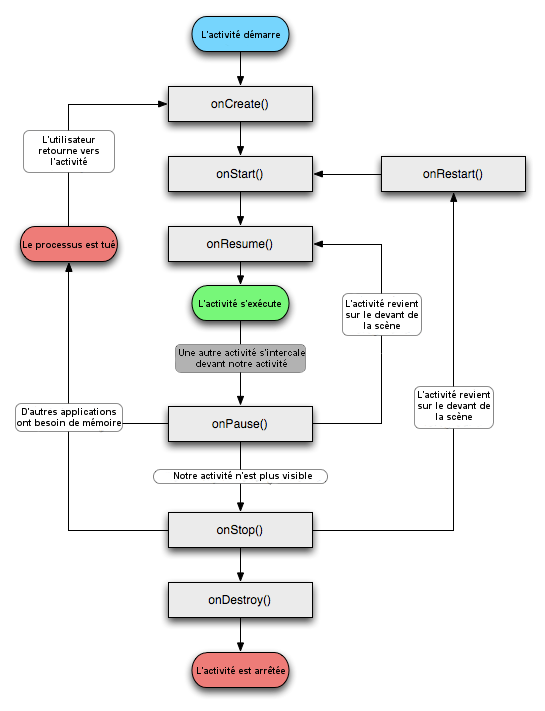
\includegraphics[height=450px]{Assets/cycleActivit_.png}
\begin{flushleft}
\hspace*{15pt}\hbox{\scriptsize Source:\thinspace{\scriptsize \itshape \url{http://developer.android.com/reference/android/app/Activity.html}}}
\end{flushleft}
\captionof{figure}{Cycle de vie d'une activité}

\label{cycleActivité}

\end{center}

Comme représenté sur le schéma, les activités peuvent avoir plusieurs états, et des méthodes de transition sont appelées en entrée et en sortie d'état.
\begin{itemize}
\item onCreate(): permet d'initialiser l'activité, avec en paramètre un objet "Bundle" qui contient des données que l'on peut lui transmettre lorsque l'activité est interrompue (comme lors de la rotation de l'écran).
\item onStart(): appelée ensuite pour charger des données.
\item onResume(): lancée lorsque l'application passe en avant-plan, soit à la première ouverture de l'activité, soit après que la fonction "onPause()" l'ait mise en arrière-plan, en prenant soin d'avoir au préalable sauvegardé l'état de l'activité à renvoyer pour "onResume()".
\item onPause(): appelée lorsque l'activité est "doublée" par une autre activité qui s'affiche par-dessus, l'activité reste affichable.
\item onStop(): intervient lors de la fermeture d'une activité, le processus se met en veille, et il pourra être relancé par la fonction "onRestart()".
\item onDestroy(): la mémoire occupée par l'activité est libérée et l'activité est supprimée de la pile d'activités.
\end{itemize}

\subsubsection{Ressources} Les ressources sont gérées sous \textit{Android} au moyen d'un objet de classe "R" qui permet d'accéder aux fichiers contenant lesdites ressources. Elles sont réparties dans différents dossiers au format XML dans le dossier "/res" du projet. 
\begin{itemize}
\item res/drawable: contient des images au format PNG, JPEG ou GIF, ou des fichiers XML contenant des directives pour dessiner des images.
\item res/layout: contient les fichiers XML décrivant la disposition d'une vue.
\item res/menus: contient les fichiers XML constituant les menus.
\item res/raw: contient des données diverses au format brute, comme des musiques ou des fichiers HTML.
\item res/values: contient diverses ressources telles que des chaînes de caractères, des dimensions, des variables,... 
\end{itemize}

\`{A} l'intérieur de ces dossiers, les ressources sont organisées en sous-dossiers représentant ce que l'on appelle des quantificateurs. Ces quantificateurs divisent ou copient une ressource de sorte quel soit adaptable à une langue ou à un appareil donné, compte tenu des informations présentes dans l'appareil. Ainsi, une application utilisée sur un portable français ira chercher ses ressources "values" dans le dossier "values-fr", et sur un portable anglais dans le dossier "values-en". Il existe divers quantificateurs afin de répartir les ressources en fonction de la taille de l'écran, sa résolution, son orientation ou encore la version de l'API.

\subsubsection{Les layouts}Les \underline{layouts} sont les fichiers XML gérant la disposition des éléments graphiques d'une activité. Ces \underline{layouts} doivent être liés à un objet de classe "Activity" dans la fonction "onCreate()". Ainsi, cette dernière pourra accéder via l'objet "R" aux composants avec lesquelles l'activité doit interagir.

\subsubsection{Le fichier AndroidManifest.xml} Ce fichier, présent pour chaque module, détaille l'ensemble des permissions que le module détient, comme le droit à l'accès au géolocaliseur du téléphone, au vibreur, aux données de l'appareil, mais aussi aux services \textit{Google}. Il contient la description des activités que le module utilisera.\\
Il contient aussi le nom du package du module, la version minimum du kit de développement que le module peut utiliser et les librairies à importer.

\subsection{Analyse de l'existant}

\textit{Google} ainsi que des développeurs indépendants ont déjà produit des applications pour l'accessibilité des personnes malvoyantes à l'évolution mobile, nous devons donc programmer en gardant cela en tête. Nous vous présentons ici quelques applications que les malvoyants peuvent utiliser sur leur téléphone de base, en essayant d'étudier ce que ces applications pourraient nous apporter ou ceux qu'on pourrait leur apporter.

\begin{itemize}
\item \textbf{TalkBack:} Application développée par \textit{Google} qui permet à l'utilisateur de se faire décrire l'écran par une voix synthétique. Cette application change le comportement du téléphone. Par exemple, le fait de cliquer sur une application ou un bouton ne valide pas l'action ciblée, mais sélectionne simplement le widget qui est alors lu par la voix synthétique. Pour valider ce widget ou bouton maintenant sélectionné, l'utilisateur a simplement à cliquer deux fois n'importe où sur l'écran.\\
Cette application qui est disponible de base sur les téléphones nous apporte un moyen de lire nos boutons aux utilisateurs, nous pouvons utiliser cette application en complément. A terme, la lecture de l'écran par une voix synthétique devrait être intégrée à l'application.
\item \textbf{Saisie vocale:} Les smartphones récents ont un microphone et une reconnaissance vocale intégrés, l'utilisateur peut donc utiliser ce moyen de saisie s'il le souhaite. Il est disponible via le bouton représentant un microphone dans le clavier virtuelle de l'appareil, ou par voix en prononçant "OK Google". Cette fonctionnalité native nous permet de ne pas avoir à l'implémenter nous-même.\\
\item \textbf{Navi'Rando\cite{Navirando}:} Dans le domaine du GPS adaptée aux aveugles, il y a \textit{Navi'Rando}, un GPS pour randonneurs malvoyants. Il guide les utilisateurs par une voix synthétique à travers les bois et les montagnes par des chemins préalablement enregistrés par les développeurs dans l'application. Ce codage des chemins "en dur" dans la base de donnée de l'application leur permet d'avoir des informations très précises à propos des obstacles des parcours, et la voix permet de les avertir de chaque obstacle qu'ils vont traverser, leur indiquer la position horaire de cet obstacle.\\
Cette application se rapproche du but de notre projet mais \textit{Navi'Rando} n'est pas un GPS discret, il préconise la précision avant la discrétion alors que nous utiliserons les vibreurs dans un souci de discrétion. De plus, nous utiliserons des itinéraires à déterminer en fonction de plusieurs paramètres, ils ne pourront donc pas être aussi précis que ceux de \textit{Navi'Rando}.
\end{itemize}

\section{Analyse des besoins de l'application}

\subsection{Besoins fonctionnels}

\subsubsection{Choix de l'environnement de programmation} Après quelques tests effectués avec \textit{Android Studio} et \textit{Eclipse} (couplé au plug-in {textit{ADT - Android Development Tools}), les deux semblent convenir pour un bon développement. \textit{Eclipse} est moins lourd à supporter pour certaines machines, mais \textit{Google} ne maintient plus le plug-in sur \textit{Eclipse}\cite{EclipseAndroid}. \textit{Android Studio} est donc utilisé. Ce dernier est développé par \textit{Google} basé sur \textit{IntelliJIDEA}, un des premiers environnements pour \textit{Java}. Il contient des fonctionnalités afin de gérer les fichier XML de layout graphiquement et intègre des outils de compilation comme \textit{Gradle} et \textit{Maven}, afin d'automatiser la création d'une application par une liste de dépendances.

\subsubsection{Android SDK 4.4 Kit-Kat} L'application sera codée en Java, couplé par le XML que nous propose l'architecture d'\textit{Android}. La version 4.4 du kit de développement d'\textit{Android KitKat} sera utilisée, afin que l'application fonctionne sur le plus d'appareils possible. Malgré tout, la version qui sera utilisée pourra en être une autre, mais toujours en préconisant la visibilité de l'application.

\subsubsection{Gestionnaire de versions, SVN} Un gestionnaire de versions va être utilisé afin de disposer d'un dépôt sur le serveur du CREMI mis à disposition aux étudiants. Nous développerons sur une copie de ce dépôt, en local, et nous validerons ces changements lorsque s'ils seront corrects. Le CREMI proposant un serveur SVN, nous utiliserons ce type de gestionnaire qui a l'avantage d'être familier aux étudiants depuis leur entrée dans l'établissement.

\subsubsection{Google Maps API } 
Afin d'utiliser les services de \textit{Google}, il a dû être nécessaire au préalable de se référencer auprès de la société via la console de développeur\footnote{\url{https://developers.google.com/?hl=fr}}. Nous avons donc précisé quel services nous allions utiliser et la console nous a alors transmis une clé d'authentification que nous devons intégrer dans le fichier "manifest" de l'application.
\paragraph{Algorithme d'itinéraire} L'interface de \textit{Google Maps Directions} sera testée. Cette dernière renvoie un fichier sous format JSON décrivant une suite de 23 points maximum (limite standard) constituant l'itinéraire calculé. Un fichier JSON est un fichier de structuration de données basé sur la syntaxe JavaScript. Il permet de représenter des informations sous formes d'arbres, comme le fait XML par exemple. Ce fichier, renvoyé par les services de \textit{Google}, contient tout un tas d'informations décrivant un chemin. Le premier niveau d'information contient les informations globales telles que la durée totale du trajet, le statut de la requête (le nombre d'itinéraires renvoyés, la validation ou non de la requête,...), les points de la ligne graphique à dessiner encodées, les points de cheminements que l'utilisateur veut particulièrement traverser et un ou plusieurs champ "route", représentant un chemin. Ce dernier contient un ou plusieurs "legs", qui eux correspondent aux chemins entre chaque point de cheminement. Ces "legs" contiennent un ou plusieurs champs "step" qui eux représentent les chemins entre chaque mouvement. Ce sont les atomes de ces itinéraires. Ils sont constitués de champs tels que "durée estimée", "prochaine manœuvre" (tourner à gauche par exemple), "point de début et d'arrivé"e et "description du step" au format HTML. Ces données sont à traiter en temps réel afin de se déplacer à travers le fichier JSON en fonction des déplacements de l'utilisateur.
\paragraph{Algorithme de géolocalisation} La géolocalisation a quant à elle une limite standard de 10 requêtes par seconde par utilisateur, dans une limite de 2500 par jour. Elle renvoie un objet de classe "Location" contenant des informations telles que la précision de la réponse, la vitesse de déplacement, la direction (en degré par rapport au Nord), le nom du fournisseur de localisation (par GPS, par WIFI ou par réseau mobile) et bien évidemment la latitude, la longitude et l'altitude du point géographique.

\subsubsection{Matériels} Les émulateurs d'appareils \textit{Android} étant très lents, le client s'engage à fournir des équipements de tests, en l'occurrence des téléphones fonctionnant sous \textit{Android}, afin de travailler dans les meilleurs conditions.\\

\subsubsection{Tests avec JUnit4}
Afin de réaliser les tests de nos fonctionnalités et de nos codes, \textit{Android SDK} fournit un module de test se nommant \textit{JUnit}\footnote{\url{http://developer.android.com/tools/testing/testing_android.html}}, la version 4 sera utilisée pour profiter au mieux du progrès de développement de \textit{JUnit}. 
\paragraph{Tests de régression} Tout les tests seront utilisés au cours du projet afin de vérifier que les nouvelles fonctionnalités apportées ne dérangent pas le bon fonctionnement des précédentes.

\subsection{Besoins non-fonctionnels}
Nous allons présenter dans cette section les besoins non-fonctionnels de l'application par module. Certains aspects expliqués ne sont pas présents dans la version du rendu final, mais nous parlerons plus en profondeur de ces points dans la partie traitant des améliorations possibles.

\subsubsection{Module de saisie d'adresse}
\paragraph{Ergonomie}
L'interface se doit d'être la plus ergonomique possible afin de permettre à un utilisateur malvoyant de naviguer dans les menus avec le plus de facilité possible. Dans l'idéal, chaque item du menu devrait faire l'objet d'une activité qui prendrait tout l'écran, il pourra aussi être envisagé de faire dicter par une boite vocale ce qu'il y a écrit. A chaque changement d'activité, le téléphone vibrera afin de signifier le changement d'activité.

\paragraph{Robustesse et stabilité}
L'ensemble des activités doit être accessible à partir des autres activités, un test doit donc être réalisé sur le graphe des activités pour vérifier qu'il est fortement connexe. Pour tester que l'application ne s'éteint pas prématurément à cause d'un bug, un oracle doit être implémenté. Cet oracle devra aléatoirement se déplaçait dans les activités afin d'augmenter la confiance en la robustesse et la stabilité de l'application.

\subsubsection{Module synchronisation}

\paragraph{Ergonomie}
Pour se synchroniser avec un autre appareil, il faut trouver un moyen efficace et simple qui fournit à un aveugle la possibilité de se connecter en \textit{BlueTooth} sans boîte vocale. Si cela est possible (les possibilités du SDK d'\textit{Android} sont à vérifier), une liste similaire à la liste des adresses devra être implémentée. Cette liste fera figure de surcouche de la boîte de dialogue d'\textit{Android}, permettant à l'utilisateur de choisir avec plus d'ergonomie l'appareil cible. Lorsqu'il aura choisi, l'appareil cible se fera reconnaître de l'utilisateur par une vibration à la demande d'appareillage, de sorte à indiquer à l'utilisateur qu'il doit maintenant appuyer sur l'écran des deux téléphones afin de valider la synchronisation.

\paragraph{Performance} Ils doivent pouvoir recevoir des ondes ou les émettre et ce, d'une rapidité convenable pour simuler un temps réel (estimé à moins d'une seconde de latence).

\paragraph{Batterie} Lorsque la batterie de l'un des deux téléphones se décharge, l'application ne sera plus en mesure de pouvoir guider l'utilisateur puisque la synchronisation sera arrêtée. La vibration sera utilisée pendant trois secondes sur le téléphone non déchargé pour indiquer à l'utilisateur que la synchronisation s'est arrêtée. L'application relancera automatiquement une nouvelle tentative de synchronisation. \emph{La recherche des appareils \textit{BlueTooth} visibles est coûteuse en énergie, elle est à faire le moins possible.}

\paragraph{Sécurité} Du point de vue sécurité, l'application serveur doit empêcher l'utilisateur malvoyant de se connecter par mégarde à un appareil tiers. Une confirmation doit donc être envoyé par le client. Également, l'application client ne doit pas laisser un appareil tiers se connecter à lui.
Les développeurs ne sont pas responsables des accidents qui surviendraient de l'utilisation de l'application sur des téléphones défectueux ou obsolètes qui créeraient des désynchronisations.

\subsubsection{Module de guidage} 
\paragraph{Performances} L'application ne doit pas afficher une localisation qui date de plus d'une seconde en mémoire, afin que le guidage soit le plus fluide possible. Les tests de performances doivent vérifier que, en moins d'une seconde, le téléphone principal reçoit les données de position et les envoie au téléphone secondaire en moins d'une seconde.

\paragraph{Capacité} L'application a un besoin constant de connexion Internet et d'une bande passante convenable qui satisfait les besoins en performance. Ces contraintes sont les mêmes en ce qui concerne la connexion \textit{BlueTooth}.

\paragraph{Disponibilité}
Afin de pouvoir utiliser l'application il est nécessaire d'avoir une connexion Internet, elle est utilisable seulement dans un lieu où le téléphone est susceptible de recevoir les données nécessaires au bon fonctionnement de celle-ci. De plus, l'application ne fonctionnera uniquement dans les lieux qui sont couverts par l'API cartographique de \textit{Google}.

\paragraph{Stabilité du code}
Des tests doivent être fournis qui permettront de certifier la bonne validité du code. 
\subparagraph{Tester les itinéraires} Le module de calcul d'itinéraire doit faire faire l'objet de tests de régression afin de certifier ses résultats.
\subparagraph{Tester les fonctions vibreur} L'application cliente doit vibrer \emph{si et seulement si} l'application serveur est à une intersection et l'itinéraire (certifié) indique la gauche ou que l'utilisateur est en sens inverse. Les mêmes tests sont requis pour l'application serveur. Quand un mauvais chemin est emprunté, les deux applications vibrent de concert un court temps avant de recalculer un itinéraire.

\paragraph{Problèmes envisagés}\subparagraph{} Pour le code à établir pour le vibreur, un simple code pour gauche ou droite ne suffira pas, car une intersection peut avoir plus de 4 routes qui s'y rattachent. Dans le cadre d'un premier prototype, et par concertation avec le client, cette éventualité sera ignorée afin de permettre en premier lieu un guidage par intersection simple.
\subparagraph{} L'application utilisant le vibreur constamment, il faut convenir d'un protocole lorsque le téléphone reçoit un appel, un message, une notification. En d'autres termes, il ne faut pas que le code vibreur soit faussé par une autre application. Là aussi, il est demandé par le client que le premier prototype ne s'occupera pas de ces possibles conflits. 

\paragraph{Sécurité}
Pour un fonctionnement optimal de l'application, l'utilisateur doit donc désactiver toute autre application pouvant utiliser le vibreur. Dans le cas contraire, l'utilisateur s'expose à des conflits qui pourrait mener à des mauvaises indications de direction, et il en sera le seul responsable. \emph{A titre informatif: Deux choix de conception sont possibles: imposer un protocole ou en laisser l'utilisateur le choix en proposant dans les paramètres un menu l'invitant à définir le comportement de l'application pour chaque événement.}

\newpage

\section{Scénarios et diagrammes}

\subsubsection{Diagramme d'états}
\begin{center}
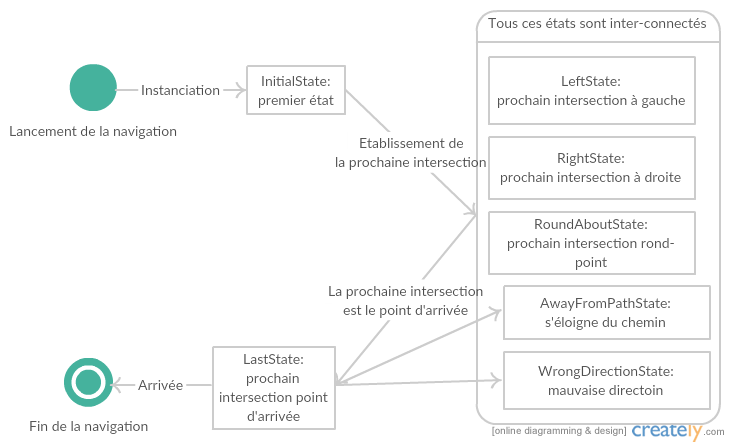
\includegraphics[height=250px]{Assets/State_navigation.png}
\captionof{figure}{Diagramme d'états en navigation}
\end{center}

\subsubsection{Diagramme de Gant}

\begin{figure}[h]
\centering
\caption{Diagramme de Gant prévisionnel}
\label{GantPrévisionel}
\begin{tabular}{llllllllllll}
\cline{1-12}
                                         \diagbox{Tâches}{Semaine} & 5 & 6 & 7 & 8 & 9 & 10 & 11 & 12 & 13 & 14 & 15 \\ \cline{1-12}
Téléchargement des cartes                 & X &   &   &   &   &    &    &    &    &    &    \\
Géolocalisation                           & X & X &   &   &   &    &    &    &    &    &    \\
Calcul d'itinéraires                      &   & X &   & X & X & X  &    &    &    &    &    \\
Mise en place de l'interface              &   & X &   & X & X & X  & X  & X  &    &    &    \\
Test de guidage basique                   &   &   & X &   &   &    & X  &    &    & X  & X  \\
Synchronisation BlueTooth                 &   &   &   & X & X & X  &    &    &    &    &    \\
Mise en place du protocole client/serveur &   &   &   & X & X & X  &    &    &    &    &    \\
Liaison vibreur / application             &   &   &   &   & X & X  & X  &    &    &    &    \\
Persistance des données                   &   &   &   &   &   &    &    & X  & X  &    &    \\
Test de guidage avancée                   &   &   &   &   &   &    &    & X  & X  & X  & X 
\end{tabular}
\end{figure}

%------------------------------

\begin{figure}[h]
\centering
\caption{Diagramme de Gant réel}
\label{GantReel}
\begin{tabular}{llllllllllll}
    \cline{1-12}                                    \diagbox{Tâches}{Semaine} & 5 & 6 & 7 & 8 & 9 & 10 & 11 & 12 & 13 & 14 & 15 \\
    \cline{1-12}
\multicolumn{12}{c}{\textbf{Module Map}}                                                   \\
\cline{1-12}
Téléchargement des cartes                & X &   &   &   &   &    &    &    &    &    &    \\
Géolocalisation                          & X & X &   &   &   &    &    &    &    &    &    \\
Requête d'itinéraire                     &   & X & X & X & X & X  &    &    &    &    &    \\
Gestion des états de navigation          &   &   &   &   &   & X  & X  & X  & X  &    &    \\
Gestion des messages vibratoire          &   &   &   &   &   & X  & X  & X  & X  &  X  &    \\
\cline{1-12}
\multicolumn{12}{c}{\textbf{Module de saisie d'adresse}}                                   \\
\cline{1-12}
Interface graphique 	 				 & X & X & X &   &   &    &    &    & X  & X  &    \\
Utilisation du Geocoder                  &   &   &   & X & X  &   &    &    &    &    &     \\
Base de données							 &   &   &   &   & X &  X &  X &    &    &    &     \\
Vérification de la connectivité réseau	 &   &   &   &   &   &    &    &  X &  X &  X &    \\
Liaison avec les deux autres modules     &   &   &   &   &   &    &    &    &    &  X &    \\ \cline{1-12}
\multicolumn{12}{c}{\textbf{Module de synchronisation}}                                    \\
\cline{1-12}
Communication socket                     &   & X & X & X & X & X  & X  & X  &    &    &    \\
Mise en place du protocole               &   &   & X &   &   &    & X  & X  & X  & X  &    \\
Liaison synchronisation/carte            &   &   &   &   &   &    & X  & X  & X  &    &    \\
Liaison synchronisation/saisie d'adresse &   &   &   &   &   &    &    & X  & X  &    &    \\
\cline{1-12}
\multicolumn{12}{c}{\textbf{Tests}} 
\\
\cline{1-12}
Test module Map							&   &   & X & X & X & X & X & X & X & X & 
	\\
Test module de synchronisation			&   &   &   &   &   &   &   & X & X & X &
\end{tabular}
\end{figure}
\newpage % Sinon l'écriture se met entre les deux tableaux
La différence de ces tableaux est dans la programmation modulaire établie après le diagramme prévisionnel. Tout les modules ont été développés parallèlement et liés entre eux une fois que les fonctionnalités étaient assez développé pour le permettre, en testant au fur et à mesure. 

\subsection{Scénarios possibles}
Pour l'utilisation de notre application, plusieurs scénarios sont possibles. Nous allons nous contenter de décrire deux scénarios possibles avec les différentes étapes.


\textbf{Scénario 1}

1. L'utilisateur démarre l'application et choisit le mode "New Itinerary"

2. L'utilisateur rentre une adresse correcte et celle-ci est enregistrée dans la base de données.

3. L'utilisateur lance l'itinéraire.

4. Le serveur est lancé en arrière-plan et est en attente de connexion entrante.

5. L'itinéraire se dessine sur la carte et la navigation commence.

6. Lorsque l'utilisateur tourne à gauche, deux vibrations sont émises.

7. Lorsque l'utilisateur tourne à droite, une seule vibration est émise.

8. Lorsque l'utilisateur marche tout droit, aucun signalement ne se fait.

9. Lorsque l'utilisateur se trompe dans l'itinéraire, il reçoit  plusieurs vibrations pour l'en avertir. S'il persiste dans la mauvaise direction, un nouvel itinéraire est calculé.

10. Enfin, lorsque l'utilisateur arrive à la destination finale, des vibrations différentes lui indique.

\begin{center}
\captionof{figure}{Diagramme de séquence 1}
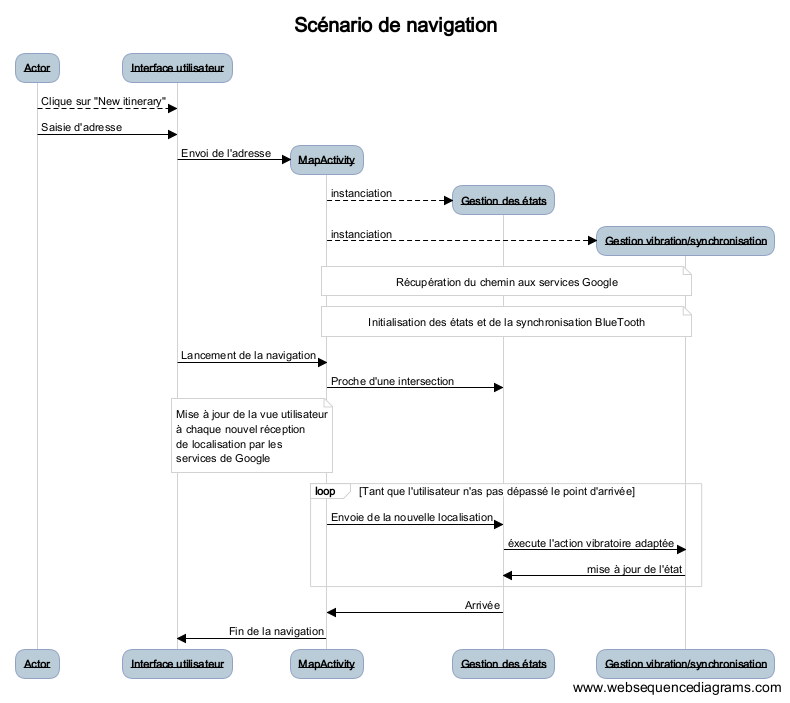
\includegraphics[height=400px]{Assets/scenario1.png}
\end{center}



\textbf{Scénario 2}

1. L'utilisateur possède deux téléphones.

2.L'utilisateur démarre l'application avec le premier téléphone et suit le scénario 1 jusqu'à l'étape 5.

3. L'utilisateur démarre l'application avec le deuxième téléphone et choisit le mode "Launch client".

4. Les deux téléphones font une tentative d'appareillement qui fonctionne.

5. Sur le premier téléphone, le choix du côté pour le lequel le téléphone qu'il tient en main doit vibrer s'affiche. Sur le deuxième téléphone, un message affiche que la connexion s'est bien passée.

6. Le choix de vibration est effectué par l'utilisateur : droite pour le premier téléphone et gauche pour le deuxième.

7. Lorsque l'utilisateur doit tourner à gauche, le deuxième téléphone vibre.

8. Lorsque l'utilisateur doit tourner à droite, le premier téléphone vibre.

9. Lorsque l'utilisateur marche tout droit, aucun signalement ne se fait.

10. Lorsque l'utilisateur se trompe dans l'itinéraire, il reçoit  plusieurs vibrations pour l'en avertir. S'il persiste dans la mauvaise direction, un nouvel itinéraire est calculé.

11. Enfin, lorsque l'utilisateur arrive à la destination finale, des vibrations différentes lui indique.

\begin{center}
\captionof{figure}{Diagramme de séquence 2}
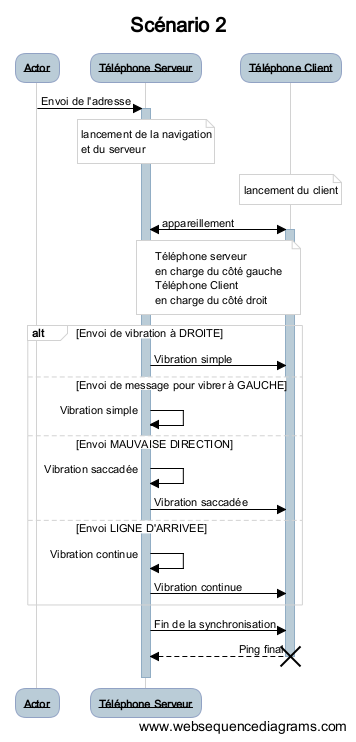
\includegraphics[height=400px]{Assets/scenario2.png}
\end{center}

\textbf{Scénario 3}

1. L'utilisateur suit le scénario 2 jusqu'à l'étape 9.

2. La synchronisation s'arrête car le serveur n'est plus connecté au client.

3. Lorsque le serveur le détecte, il passe directement en mode solo.

4. Le téléphone serveur continue le scénario 1 à partir de l'étape 6. 

\begin{center}
\captionof{figure}{Diagramme de séquence 3}
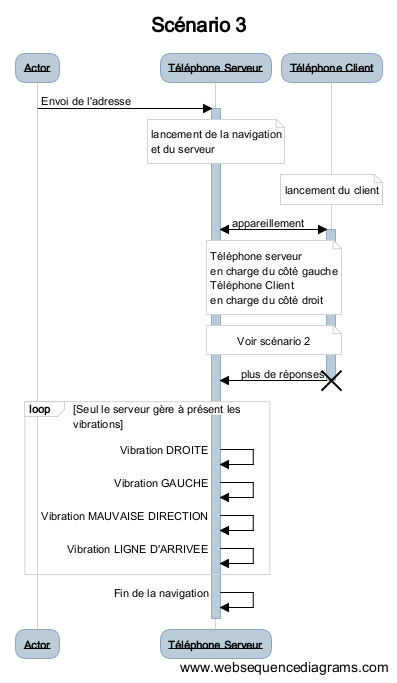
\includegraphics[height=400px]{Assets/scenario3.png}
\end{center}

\textbf{Scénario 4}

1. L'utilisateur suit le scénario 2 jusqu'à l'étape 9.

2. La synchronisation s'arrête car le client n'est plus connecté au serveur. Le client n'a pas reçu d'acquittement du \emph{ping}.

3. Lorsque le client le détecte, il utilise l'adresse qu'il a reçu préalablement du serveur pour continuer l'itinéraire en mode solo. 

\begin{center}
\captionof{figure}{Diagramme de séquence 4}
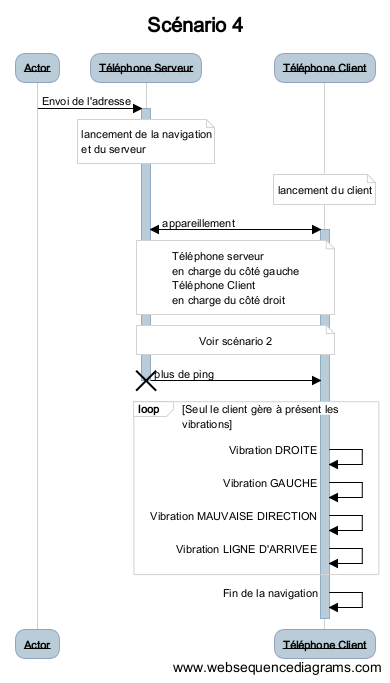
\includegraphics[height=400px]{Assets/scenario4.png}
\end{center}





\chapter{Architecture et description de l'application}

\section{Architecture des modules}
\begin{center}
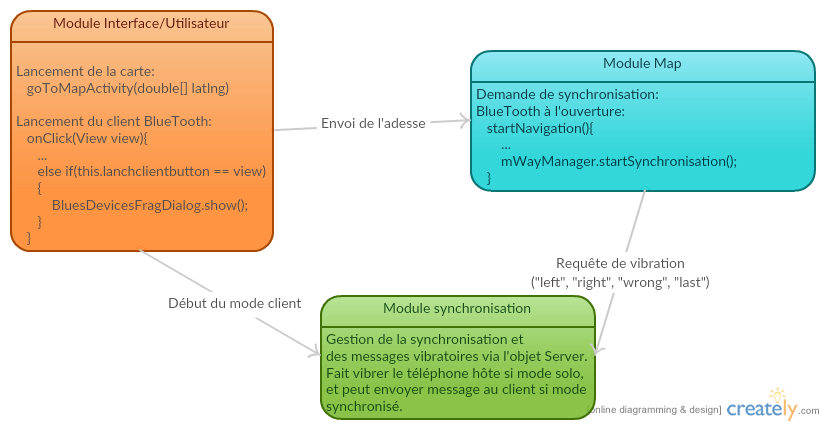
\includegraphics[height=250px]{Assets/Lien_entre_modules.png}
\begin{flushleft}
\hspace*{15pt}\hbox{\scriptsize Source:\thinspace{\scriptsize \itshape \url{http://www.creately.com}}} % Inutile de mettre une source d'un dessin que tu as fait toi-même
\end{flushleft}
\captionof{figure}{Lien entre les modules}
\label{LienModule}
\end{center}
L'application GPS pour les malvoyants est composée de 3 modules : un module "Map" qui manipule les cartes et la navigation, un module "Synchronisation" qui est en charge du protocole de communication \textit{BlueTooth} entre les deux téléphones portables et un module "UI" qui représente l'interface utilisateur (accueil de l'application et saisie d'adresse).

\subsection{Module de saisie d'adresse}
\label{subsec:ModuleUI}
\subsubsection{Description générale}
\begin{center}
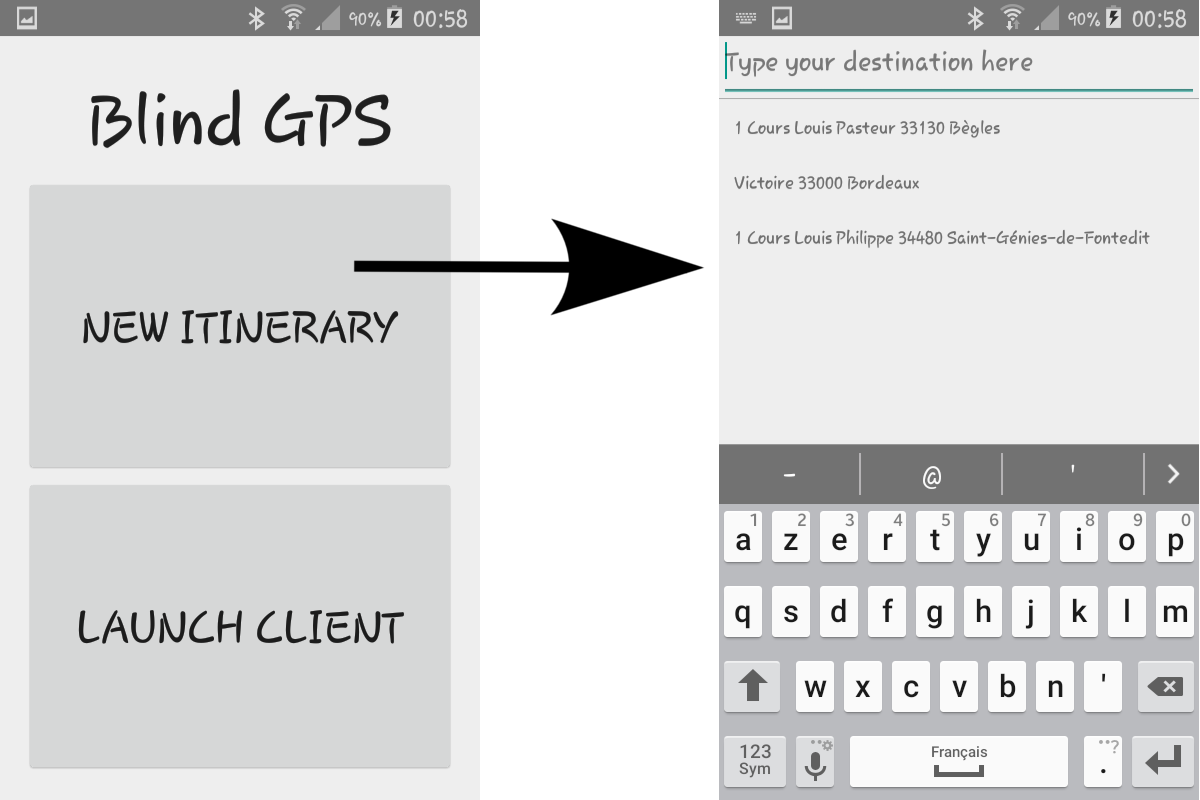
\includegraphics[height=250px]{Assets/screenUI.png}
\captionof{figure}{Capture d'écran de l'ouverture de l'application vers la saisie d'adresse
}
\label{screenUI}
\end{center}
Étant donné que l'application est destinée à un malvoyant, l'interface graphique doit être la plus simple et la plus intuitive possible. Elle est organisée en deux activités, une activité d'accueil et une activité permettant la saisie ou la sélection d'une adresse puis la transition vers le module de navigation. L'activité d'accueil est composée d'un titre, soit le nom de l'application et de deux gros boutons. Le premier bouton permet de démarrer un itinéraire, c'est-à-dire de passer à l'activité de saisie d'adresse, le second bouton permet quant à lui le lancement du couplage \textit{BlueTooth} avec le second appareil. La seconde activité, est composée d'une barre de saisie permettant de saisir l'adresse de destination. A cela s'ajoute en dessous, une liste des dernières destinations utilisées, permettant d'éviter une saisie redondante. De plus, lorsque l'utilisateur entre l'adresse de destination souhaitée, une liste de suggestions vient remplacer la liste des entrées récentes et se met à jour au fur et à mesure que la tape au clavier progresse. Enfin, afin de se différencier d'un GPS classique et de s'adapter au problème de vue de l'utilisateur, une saisie vocale est disponible, et lors de la validation de l'adresse cible, cette dernière est lue par une voix synthétique confirmant l'adresse saisie dans le but de permettre à l'utilisateur de savoir s'il s'est trompé ou non dans l'adresse validée.

\subsubsection{Diagramme des classes}
\begin{center}
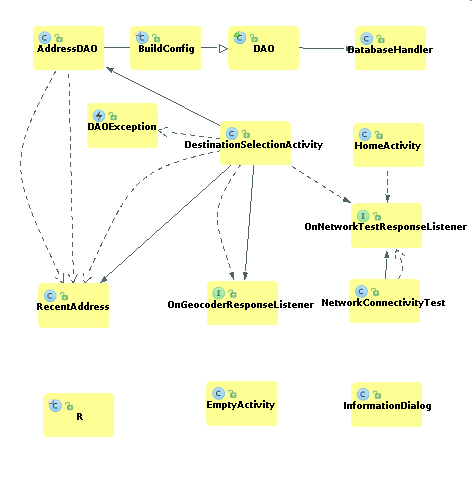
\includegraphics[height=250px]{Assets/uiUML.png}
\captionof{figure}{Diagramme des classes du module UI\\
Flèches à pointe pleine: référence sur, en donnée membre.\\
Flèches à pointe creuse: étend la classe pointée.\\
Flèches pointillées à pointe creuse: implémente la classe pointée.\\
Flèches pointillées à pointe pleine: référence sur, en variable locale à une méthode.}
\label{uiUML}
\end{center}

\subsubsection{Description technique}

\begin{itemize}
\item \textbf{Classe HomeActivity :} lors du lancement de l'application, l'activité "HomeActivity" est affichée (donc ajoutée en haut de la pile des activités). Lorsque l'on clique sur le bouton "New itinerary", la connexion réseau est vérifiée grâce à l'objet "NetworkConnectivityTest" qui vérifie la connectivité réseau. Une fois le test réseau passé, l'activité "DestinationSelectionActivity" est lancé (ajouté au-dessus de l'activité précédente dans la pile des activités). Si le test échoue (application non reliée à Internet), un message d'erreur est affiché indiquant la nécessité d'être connecté à Internet.\\ Pour ce qui est y du clic sur le second bouton, "Launch client", il affiche une boîte de dialogue "BlueDevicesDialogFrag" présente dans le module "Synchronisation" qui permet la sélection de l'appareil \textit{BlueTooth} avec lequel se coupler.\\

\item \textbf{Classe DestinationSelectionActivity :} au lancement de l'activité "DestinationSelectionActivity", un thread est lancé en tâche de fond qui permet d'effectuer des requêtes grâce à l'objet "Geocoder" pour obtenir des suggestions d'adresses. La classe "Geocoder" est une classe native de l'API \textit{Android} permettant la récupération d'adresses postales, et leurs informations associées, dont la longitude et la latitude, utilisées pour la navigation. Ainsi, à chaque nouveau caractère tapé dans la barre d'entrée d'adresse, une requête est soumise au thread "GeocoderDialog" et une requête de suggestions est envoyé. A la réception des nouvelles suggestions, la liste des suggestions est mise à jour via la fonction "onGeocoderResponse()" (\underline{pattern Listener}). Après avoir obtenu aperçu dans la liste des suggestions, l'adresse de destination souhaitée, l'utilisateur sélectionne la suggestion et amorce ainsi la méthode "callback" "onTouch()". En premier lieu, l'adresse sélectionnée est récupérée via un unique identifiant dans la liste. Puis, elle est insérée dans la base de donnée, grâce à l'objet "AddressDAO" et la méthode "insert()". Si elle n'était pas présente dans la base, elle est insérée normalement, si c'était le cas, son compteur d'utilisations et sa date de dernière utilisation (ce qui permet de classer les entrées récentes par date de dernière utilisation) sont simplement mis à jour. Ensuite,l'adresse est lue via l'objet "TextToSpeech", qui permet une synthèse vocale, si la fonctionnalité est supportée par l'appareil. Enfin, la méthode "goToMapActivity()" est lancé et permet la transition vers l'activité de navigation tout en lui passant la longitude et la latitude de l'adresse sélectionnée.\\
L'utilisateur peut aussi être exempté de tape au clavier redondante s'il a déjà tapé cette adresse auparavant. Grâce à la base de données, les entrées récentes sont affichées (classées de la plus récente à la moins récente) et il n'a plus qu'à simplement sélectionner celle désirée. Dans ce cas précis, la date de dernière utilisation et le compteur d'utilisations sont juste mis à jour grâce à la fonction "update()" dans la base de données.\\
{\it \underline{Note d'implémentation :} il est aussi important de souligner que l'utilisation d'un thread en tâche de fond pour les requêtes vers le "Geocoder" permet de soulager le thread UI (thread principal de l'application) de l'attente des réponses et par conséquent de fluidifier la tape au clavier dans le champ d'adresse. Aussi, si on regarde la méthode "callback" "onGeocoderResponse()" :}

\begin{lstlisting}
@Override
public void onGeocoderResponse(final List<Address> addresses) {
    new Handler(getMainLooper()).post(new Runnable() {
        @Override
        public void run() {
            suggestionsListData = addresses;
            displaySuggestions();
        }
    });
}
\end{lstlisting}

{\it on remarque qu'on fait appel à un objet "Handler" qui envoie (méthode "post()") un objet "Runnable" à la boucle principale (le thread qui gère les éléments graphiques entre autres). Tout ceci signifie en fait qu'on indique à la boucle principale d'exécuter la fonction "run()" à la place du thread courant. Car dans un système Android, il y a une contrainte de modification sur les éléments graphiques, seul le "thread UI" (boucle principale) peut modifier ses éléments graphiques. Nous sommes donc obligés de lui faire mettre à jour sa liste de suggestions par lui-même.}\\

\item \textbf{Classe NetworkConnectivityTest :} permet d'effectuer un test de connectivité réseau. Tout d'abord, le statut de l'interface réseau du téléphone est vérifié pour savoir si une connexion (\textit{Wifi} ou réseau mobile) est active. Ensuite, un "ping" de test vers le serveur "google.com" est envoyé pour être sûr d'être bien connecté à Internet. Cette classe étend la classe "AsyncTask" (fonctionnement détaillée dans le module de navigation), ce qui lui permet de lancer une tâche de fond. En effet, pendant toute la durée du "ping", une boîte de dialogue "ProgressDialog" est affichée indiquant à l'utilisateur de patienter (avec un "spinner" d'attente). Une fois, le test effectué (dure en général moins d'une demi-seconde), la boîte de dialogue est révoquée et la fonction "callback" "onNetworkTestResponse()" du "client" du test (le "listener") est appelée, ce qui signifie qu'il doit implémenter l'interface "OnNetworkTestResponseListener" et avoir réécrit le "callback" "onNetworkTestResponse()" qui lui permet d'obtenir la réponse du test de manière asynchrone.\\

\item \textbf{Classe InformationDialog :} représente une boîte de dialogue qui indique que l'application doit être connecté à Internet pour fonctionner. Elle est créée et affichée lorsque le test réseau échoue ou lorsque la requête de suggestion n'aboutit pas (à cause de l'absence de connexion réseau).\\
\end{itemize}

Les deux interfaces suivantes permettent d'implémenter le \underline{pattern "Listener"} et contiennent une méthode "callback" (très utilisée dans le système \textit{Android}) appelée lors d'un événement.\\

\begin{itemize}
\item \textbf{Interface OnGeocoderResponseListener :} permet la récupération des suggestions du "Geocoder". Une classe utilisant le "Geocoder" doit implémenter cette interface et en réécrire la méthode "onGeocoderResponse()" pour traiter les suggestions obtenues. 
\item \textbf{Interface OnNetworkTestResponseListener :} permet la récupération du résultat du test de connectivité réseau. Une classe qui teste la connexion réseau doit implémenter cette interface et en réécrire la méthode "onNetworkTestResponse()" pour obtenir le booléen représentant si oui ou non on est bien connecté à Internet.
\end{itemize} 

\subsubsection{Stockage des données}

Afin de stocker les entrées récentes de l'utilisateur de l'application dans le but de lui faire gagner du temps, une base de donnée SQSLite\footnote{\url{https://www.sqlite.org/}}, qui est implémenté nativement dans le SDK \textit{Android}, a été mise en place. Elle permet l'ajout, la suppression et la mise à jour d'adresses utilisées par l'utilisateur. L'implémentation suit le \underline{pattern "DAO"} ("Data Access Object") dont je me suis fortement inspiré sur le tutoriel d'\textit{OpenClassrooms}\cite{BDD}.

\begin{itemize}
\item \textbf{Classe DatabaseHandler :} cette classe permet la manipulation de la base de données du mobile, elle étend la classe "SQLiteOpenHelper" qui est la classe native qu'il faut étendre pour pouvoir toucher à la base de données. Grâce à l'objet "SQLiteDatabase", on peut y ajouter ou supprimer des tables. La méthode "onCreate()" est appelée à la première utilisation de l'application et la méthode "onUpgrade()" lors d'une mise à jour de l'application (reset des tables).\\
\item \textbf{Classe abstraite DAO :} elle permet la manipulation de la base de données d'un point de vue de l'application, elle gère un objet "DatabaseHandler" et propose des méthodes génériques (ouverture en écriture, ouverture en lecture, fermeture, obtention). Cette classe doit obligatoirement être étendu pour spécifier des méthodes qui manipuleront les tables.\\
\item \textbf{Classe AddressDAO :} comme expliqué précédemment, c'est la classe qui va contenir les méthodes spécifiques à la table "RecentAddresses" et étendre la classe "DAO". Elle manipule l'objet "SQLiteDatabase" (qui représente une base de donnée ouverte en écriture dans ce cas) et utilise les méthodes de cette objet pour modifier la table (insertion, suppression, modification, obtention d'entrées). Si une erreur survient lors d'une manipulation, une exception "DAOException" est levée.\\
\item \textbf{RecentAddress :} structure de données représentant une adresse utilisée par l'utilisateur et sauvegardée dans la base de données. Les suggestions sont représentées par cette objet, ils sont créés lors de la récupération de la liste de suggestions depuis la base de données. Cette structure contient un identifiant unique et un intitulé, qui seront assignés aux "views" graphiques les représentant, un compteur d'utilisations et une date de dernière utilisation. Étant donné que cette structure étend la structure de données native "Address", elle possède aussi une longitude et une latitude qui seront utiles pour la navigation.
\end{itemize}

\newpage
\subsection{Module de gestion de cartes et de navigation}

\subsubsection{Description générale}

\begin{center}
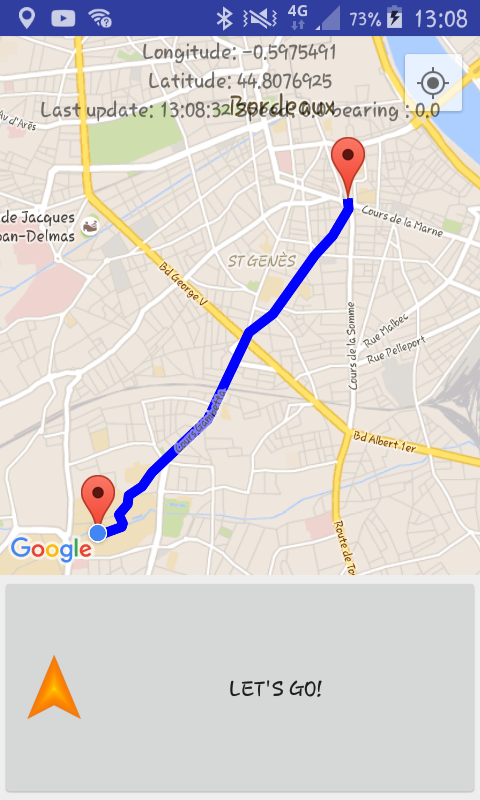
\includegraphics[height=250px]{Assets/screenMap.png}
\captionof{figure}{Capture d'écran de l'écran de carte}
\label{screenMap}
\end{center}

Une fois que l'utilisateur a saisi une adresse, la carte s'affiche et dessine l'itinéraire à partir de la position courante jusqu'à la destination entrée. L'utilisateur a accès à un bouton en haut à droite de l'écran afin de centrer la caméra sur sa position, et un plus gros bouton en bas de l'écran afin de lancer la navigation. Lorsque l'utilisateur clique sur ce bouton, la caméra se place derrière le curseur de position et l'application va maintenant faire vibrer le ou les téléphones.\\
Quand aucun autre téléphone n'est couplé, il est en mode solo, c'est-à-dire qu'il vibrera une fois pour aller à droite et deux fois pour aller à gauche lorsqu'il s'approchera d'une intersection. Lorsque un téléphone se connecte (Voir section \ref{subsec:ModuleUI}),la navigation passe en mode synchronisation, c'est-à-dire que l'utilisateur va pouvoir choisir, au moyen d'une boite de dialogue, quel téléphone sera délégué de vibrer à droite. \\Dans les deux modes, d'autres messages vibratoires lui seront envoyés. Quand l'utilisateur est sur le bon trajet mais qu'il avance dans le sens inverse, des vibrations saccadées lui indiqueront à intervalles réguliers jusqu'à ce qu'il fasse demi-tour. Quand il s'éloigne du chemin, des vibrations saccadées sont aussi transmises mais, différentes de celles du mauvais sens et l'application recalculera un nouvel itinéraire quand il sera trop éloigné. Enfin, une vibration continue lui indiquera quand il sera prêt ou sur le point d'arrivée. 

\newpage
\subsubsection{Diagramme des classes}
\begin{center}
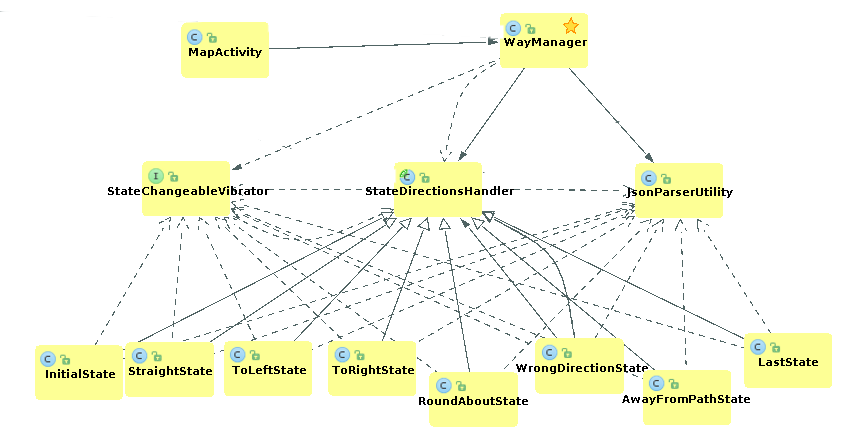
\includegraphics[height=250px]{Assets/mapUML.png}
\captionof{figure}{Diagramme des classes du module Map\\
Flèches à pointe pleine: référence sur, en donnée membre.\\
Flèches à pointe creuse: étend la classe pointée.\\
Flèches pointillées à pointe creuse: implémente la classe pointée.\\
Flèches pointillées à pointe pleine: référence sur, en variable locale à une méthode.}
\label{mapUML}
\end{center}

\subsubsection{Description technique}

Nous allons présenter les différentes classes les plus importantes au fonctionnement de ce module, en passant par l'activité qui contient tout jusqu'aux classes gérant les différents états.
\paragraph{Gestion de la carte et de l'itinéraire}

\begin{lstlisting}
public class MapActivity extends FragmentActivity
        implements OnMapReadyCallback, GoogleApiClient.ConnectionCallbacks, GoogleApiClient.OnConnectionFailedListener, LocationListener 
\end{lstlisting}

Cette classe contient la seule activité du module et implémente les différentes interfaces afin de communiquer avec les services \emph{Google}. En instanciant un objet de classe "GoogleApiClient", qui est le point d'entrée aux services, elle récupère la carte du monde, contient des méthodes "callbacks" de connexions afin de traiter une éventuelle perte de signal et contient aussi les méthodes pour récupérer la position courante. Des fonctions de requêtes d'activation de connexion Internet lui sont aussi déléguées afin de demander à l'utilisateur d'activer sa connexion si celle-ci n'est pas active.

\begin{lstlisting}
public class WayManager extends AsyncTask<Void,Void,Void> implements Parcelable, StateChangeableVibrator
\end{lstlisting}

Cette classe, contenue par "MapActivity", est en charge des comportements de l'application lorsque l'utilisateur est en navigation. Elle est instanciée dès que "MapActivity" est connectée, par la fonction "onConnected()" de l'interface "ConnectionCallBacks". Elle étend la classe "AsyncTask<Params, Progress, Result>" qui est une classe permettant de lancer des actions généralement longues en tâche de fond à l'appel de la méthode "execute()" par trois méthodes à redéfinir:
\begin{itemize}
\item onPreExecute(): méthode appelée sur le thread courant avant que la tâche ne soit exécutée. Elle est en général utilisée pour instancier les données utiles au bon déroulement de la tâche.
\item doInBackground(Params...): méthode qui lance un nouveau thread dès que "onPreExecute()" est terminée et qui exécute son implémentation en tâche de fond.
\item onPreExecute(Result...): méthode directement appelée sur le thread appelant à la fin de la tâche de "doInBackground()".
\end{itemize}
"WayManager" est la classe qui envoie une requête HTML aux services \textit{Google} afin de demander le meilleur itinéraire, et ceci est une action potentiellement très longue. C'est pourquoi il a été choisi de lancer une fenêtre modale dans "onPreExecute()" et de bloquer l'application jusqu'à ce que doInBackground() ait fini de récupérer le fichier JSON qui décrit l'itinéraire, et que "onPostExecute()" ferme la fenêtre modale.\\
C'est aussi la classe qui dessine sur la carte l'itinéraire, qui gère les mouvements de caméra et qui gère le lien avec le module de synchronisation. Pour ce dernier point, elle contient des méthodes pour commencer la synchronisation et la terminer, mais aussi des méthodes d'envoi de messages aux modules. Elle enverra par exemple au module synchronisation l'information "gauche" pour indiquer qu'il doit faire vibrer pour tourner à gauche, selon le mode "solo" ou le mode "synchronisé" que "WayManager" n'a pas besoin de connaître.\\
Elle possède une méthode "event(Location location, boolean onWay)" qui est appelée par "MapActivity" à chaque fois que la localisation change, et qui est en charge de mettre à jour les objets d'états que nous décrirons plus loin.

\begin{lstlisting}
public class JsonParserUtility implements Parcelable
\end{lstlisting}

Cette classe est celle qui récupère et traite l'itinéraire sous format JSON. Elle est codé à l'aide de l'objet "JSONParser" fourni par le kit de développement \textit{Android}. En réalité, c'est les actions de cette classe qui sont exécutées dans l'action en tâche de fond de \textit{WayManager}. Elle récupère le fichier, vérifie son intégrité et permet d'accéder aux champs par des méthodes qui simplifie sa lecture. 

\paragraph{Gestion des états}
Pendant la navigation, l'application doit pouvoir gérer plusieurs états, à savoir: quand l'utilisateur doit tourner à gauche à la prochaine intersection, à droite, quand il est dans le mauvais sens, quand il s'éloigne de la route, quand il s'approche d'un rond-point et quand il s'approche de la ligne d'arrivée. Dans un souci de maintenabilité et de bonne lecture du code, le patron de conception \underline{État} paraît bien adapté à la situation. Une classe abstraite a été implémentée:

\begin{lstlisting}
public abstract class StateDirectionsHandler implements Parcelable
\end{lstlisting}

C'est dans cette classe que l'essentiel des points algorithmiques de navigation sont implémentés.\\Pour une première approche, nous avons développé une fonction permettant de trouver l'angle entre le point courant, la prochaine intersection et celle d'après, en utilisant la \underline{loi des cosinus}. Un angle entre 0 et 120 degrés (valeurs définies statiquement dans cette classe) indiquera que l'utilisateur doit tourner à gauche dans 5 mètre (valeur également définie en tant que constante). Mais, le fichier JSON nous donnant une liste des manœuvres pour chaque point, il nous a paru judicieux de changer d'implémentation et de simplement lire le fichier pour trouver quel est le prochain état. La fonction qui utilisait la \underline{loi des cosinus}, initialement appelée "findNextState(LatLng location)", est finalement renommée "RoundAboutExit(LatLng location)" car elle servira au passage des rond-points. En effet, ceux-ci sont simplement notés dans le fichier JSON "roundabout-right" avec seulement le numéro de la sortie (3th, 1st,...) sans localisation, nous allons donc avoir besoin de cette fonction pour déterminer quand l'utilisateur approche de la sortie.\\
Elle contient aussi des fonctions permettant de traiter les données de localisation pour déterminer si l'utilisateur est dans la mauvaise direction et pour récupérer les points de la ligne dessinée que l'utilisateur doit suivre.

\newpage
\subsection{Module de synchronisation Bluetooth}

\subsubsection{Architecture Client/Serveur}
L'application GPS pour les malvoyants utilise une architecture Client/Serveur. Deux téléphones sont nécessaires pour cela. L'un servira de serveur et le deuxième téléphone sera le client.

Le téléphone serveur sera celui qui affichera la carte, l'itinéraire et la position de l'utilisateur sur la carte. Il est sensé vibrer pour le coté qui lui aura été choisi par l'utilisateur. Par défaut, le téléphone serveur vibre pour le coté droit.

Le téléphone client ne fait qu'exécuter ce que le téléphone serveur lui demande. Il est sensé se connecter au téléphone serveur via la boîte de dialogue qui affichera un ensemble de serveurs éventuels. Ce téléphone vibre pour le coté gauche mais l'utilisateur pourra éventuellement le modifier.

\subsubsection{Protocole de communication}
Le premier téléphone qui se connecte à l'application choisit l'option de démarrer l'application en mode "solo", c'est à dire sans synchronisation. Ce mode permet d'utiliser l'application sans faire appel à un autre téléphone. Dans ce cas, nous utilisons le protocole avec les vibrations mentionné ci-dessus dans la partie des besoins (cf besoins).

Lorsqu'un deuxième téléphone est amené à être utilisé, le deuxième téléphone devra se mettre en mode synchronisation. En sélectionnant ce mode, une boîte de dialogue proposant un ensemble de téléphones auxquels le deuxième téléphone pourra se connecter. Dès lors que les téléphones essayent de se coupler pour la première fois, une boîte de dialogue s'affiche sur les deux téléphones et demandent ainsi l'appareillement. Si l'appareillement a déjà eu lieu une première fois, les fois suivantes, cette boite de dialogue de demande d'appareillement ne s'affichera plus tant qu'ils restent dans la liste des téléphones appareillés pour l'un et pour l'autre.

En cas de déconnexion lors d'une synchronisation, le téléphone délaissé, se mettra directement en mode "solo".
 

\subsubsection{Fiabilité du protocole}
La connexion entre deux téléphones utilisant l'application est entièrement sécurisée. En effet, l'utilisation d'un identifiant unique de connexion (UUID) garantit une connexion qu'entre les téléphones ayant cet identifiant. C'est grâce à cette clé (UUID) que les deux téléphones s'assurent qu'ils se sont connectés dans le cadre de l'utilisation du GPS.
Par cette méthode, seuls les téléphones ayant installés l'application pourront se coupler pour faire usage de l'application.

Le téléphone serveur est apte à détecter une déconnexion du téléphone client qui lui envoie un "ping" toutes les 5 secondes. Lorsque le téléphone serveur ne reçoit plus de "ping", il se passe directement en mode solo car la synchronisation n'est plus établie. Elle peut être relancée par l'utilisateur s'il est à l'origine de cette interruption.

Lorsque le téléphone client détecte l'absence de connexion avec le téléphone serveur car ce dernier ne lui a pas envoyé de "ping" d'acquittement, il se lance en mode solo avec les informations que le téléphone serveur lui aurait communiqué.

\subsubsection{Diagramme des classes}
\begin{center}
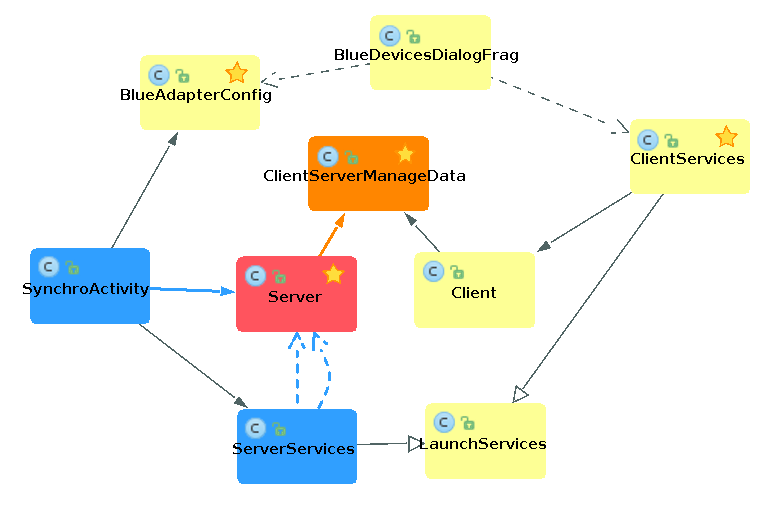
\includegraphics[height=300px]{Assets/synchroUML.png}
\captionof{figure}{Diagrammes de classes du module Synchronisation\\
Flèches à pointe pleine: Référence sur, en donnée membre.\\
Flèches à pointe creuse: Étend la classe pointée.\\
Flèches pointillées: Référence sur, en variable locale à une méthode.}
\label{synchroUML}
\end{center}

\subsubsection{Description technique}

Le module synchronisation gère le cas de l'utilisation de deux téléphones. Il est composé principalement des classes suivantes:

\begin{lstlisting}
public class BlueAdapterConfig implements Parcelable 
\end{lstlisting}

C'est cette classe qui initialise l'adaptateur \textit{Bluetooth}, l'ensemble des appareils auxquels il peut s'appareiller et met en place un ensemble de fonctions comme celle de l'activation du \textit{Bluetooth} avec "enableVisibility()" ou encore celle de recherche des appareils environnants avec "find()".

\begin{lstlisting}
public class BlueDevicesDialogFrag extends DialogFragment
\end{lstlisting}

La classe "BlueDevicesDialogFrag" intervient principalement lorsqu'on lance le mode "synchronisation". Une boîte de dialogue avec l'ensemble des appareils \textit{Bluetooth} visibles. Après sélection de l'appareil serveur dans la liste, le client est créé et la tentative de connexion commence. Une fois le client connecté, un "toast" s'affiche pour indiquer au client que la connexion s'est bien établie.

\begin{lstlisting}
public class Client extends Thread 
\end{lstlisting}

Cette classe sert principalement pour la création d'un nouveau client, c'est à dire un appareil qui tente de se connecter à un autre. Le client envoie toutes les 5 secondes un "ping" au serveur pour que le serveur sache qu'il est toujours connecté ou non.

\begin{center}
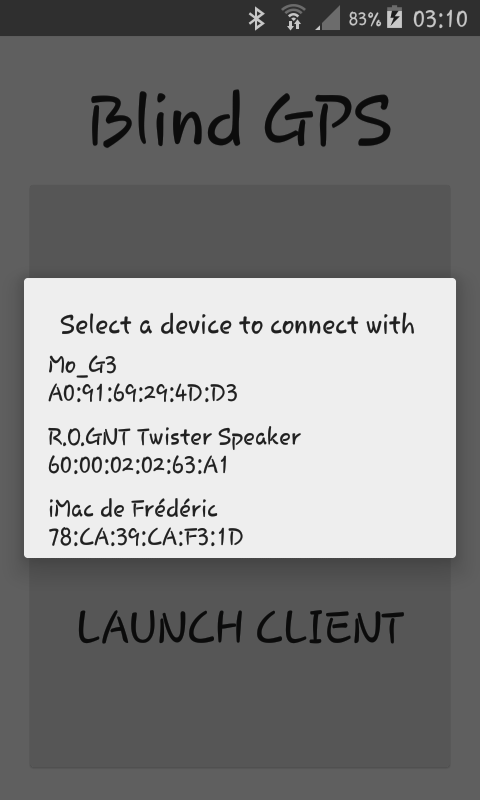
\includegraphics[height=250px]{Assets/client.png}
\captionof{figure}{Capture d'écran de lancement du client}
\end{center}

\begin{lstlisting}
public class Server extends Thread implements Parcelable 
\end{lstlisting} 

Dans cette classe, il est question de la création du serveur, qui représente l'appareil auquel on se connecte. Le serveur accepte la connexion d'un client et lui envoie des messages à travers l'objet "BluetoothSocket". Une fois la connexion établie, le téléphone serveur se voit proposé de choisir s'il veut vibrer pour la gauche ou pour la droite.

\begin{center}
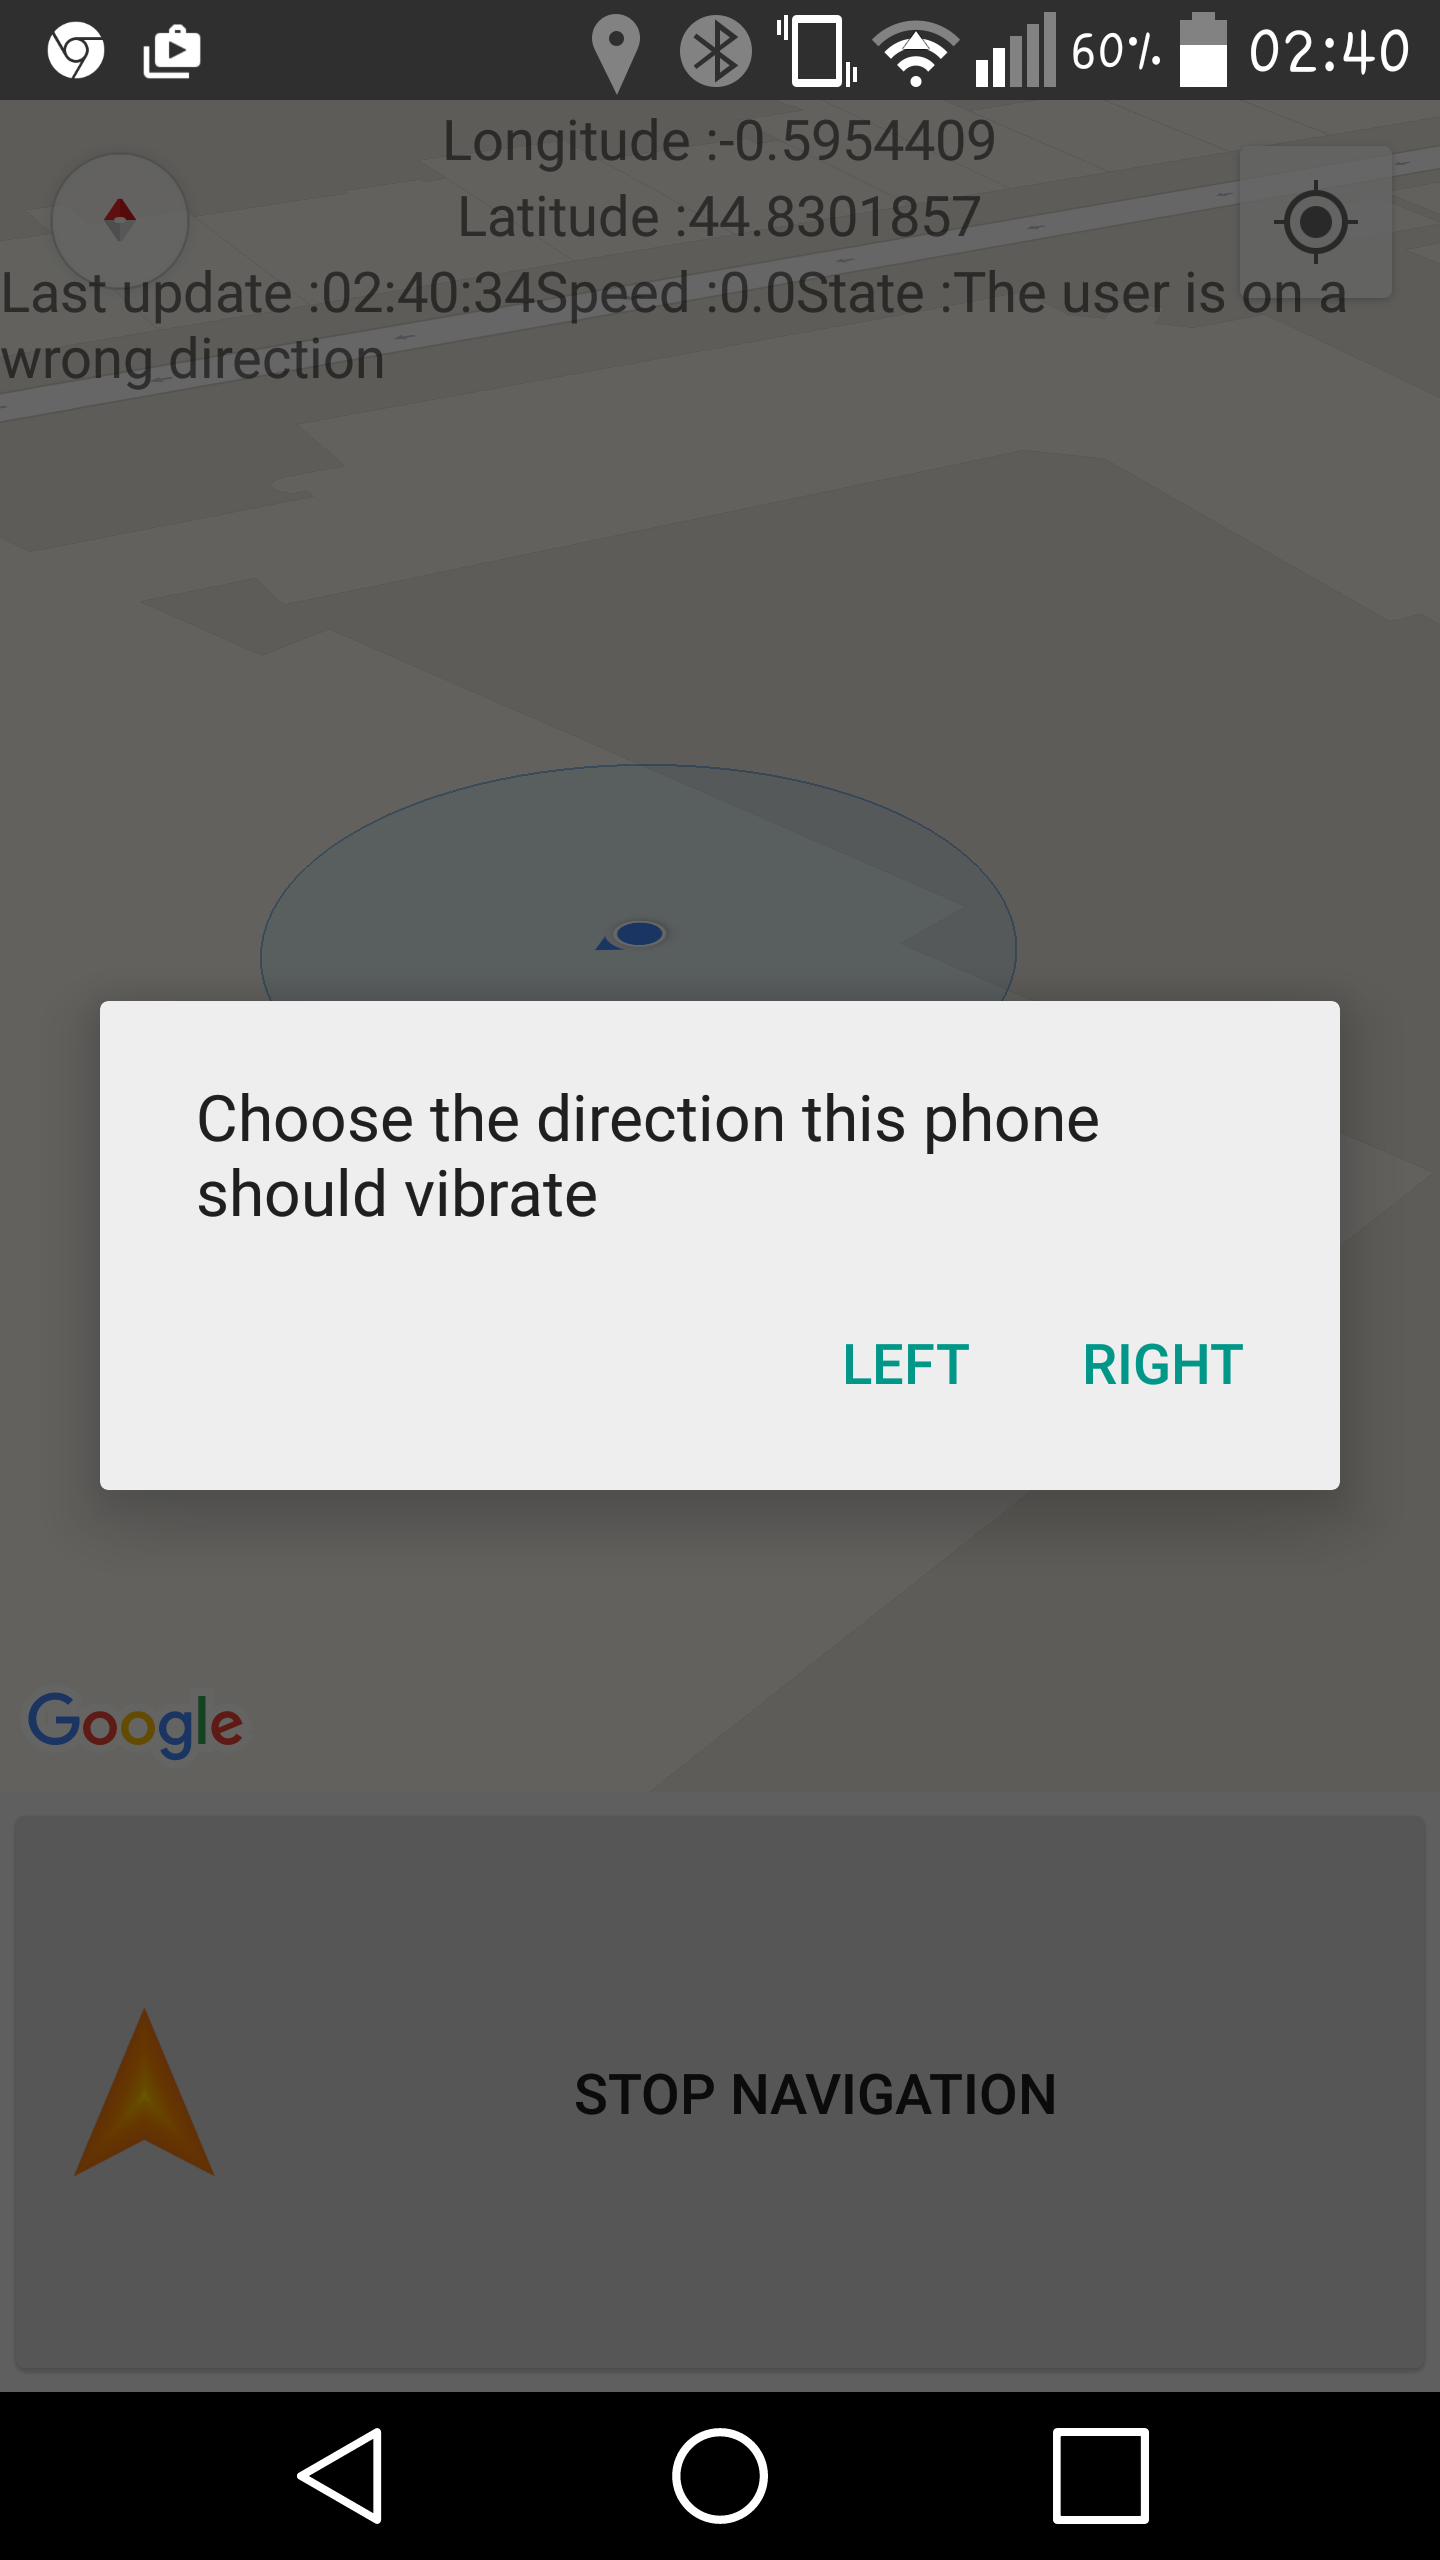
\includegraphics[height=250px]{Assets/Server.png}
\captionof{figure}{Capture d'écran de lancement du serveur}
\end{center}

Après le choix de l'utilisateur, un booléen est mis à jour afin de faire le traitement des messages échangés avec la fonction "writeblue()": 

\begin{lstlisting}
 public void writeBlue(String bytes) {
        if (blueSocket!=null && blueSocket.isConnected()) {
            if((bytes.equals("right") && posRight==true)
            || (bytes.equals("left") && posRight==false))
                vibrator.vibrate(1000);
 [...]
\end{lstlisting} 

\begin{lstlisting}
public class ClientServerManageData extends Thread 
\end{lstlisting}

Dans cette classe, ce sont les traitements des échanges de données entre le client et le serveur qui sont exécutés. Toute donnée entrante ou sortante d'une "socket" passe par cette classe.
Dans cette classe, on détecte aussi la déconnexion d'un client ou d'un serveur grâce aux "pings" ou aux acquittements dans la méthode "run()".

\begin{lstlisting}
[...]
  while (blueInStream.available() < 1) {
                    fin = System.currentTimeMillis();
                    timePing = fin - debut;
                    if (timePing > 9000) {
                        blueInStream.close();
                        blueOutStream.close();
                        blueSocket.close();    
                    }
[...]                    
\end{lstlisting}

Grâce à ce code, il est possible de faire en sorte que le client se mette en mode solo car il n'est plus connecté au serveur.
\chapter{Tests}

\section{Tests unitaires}

Afin de rendre nos modules sûrs et prêts à l'intégration, nous avons décidé de créer des tests sur la majorité de nos méthodes (certaines méthodes nécessitant des fonctions propres aux smartphones sous \textit{Android}, nous n'avons donc pas pu les vérifier en effectuant des tests unitaires). Le principal intérêt est de s'assurer que le code répond toujours aux besoins même après d'éventuelles modifications. Pour ce faire, nous utilisons un outil intégré à \textit{Android Studio}, qui s'appelle \textit{JUnit}. C'est un framework spécialisé dans le développement des tests unitaires reposant sur des assertions qui testent les résultats attendus. Nous usons aussi d'un outil permettant d'aller plus loin dans nos tests, cet outil est \textit{Mockito}. Mais l'utilisation de ce dernier est relativement compliquée et limitée dans un environnement \textit{Android}.


\subsection{Utilisation de JUnit}

\textit{JUnit} s'est avéré être un bon outil dans la mise en place de tests unitaires simples, algré un début un peu difficile pour comprendre toutes les subtilités. Tout d'abord, nous avons décidé de mettre comme convention un nom de classe de ce modèle: "[nom de la classe à tester]Test" et pour les méthodes testées les noms seront de ce modèle: "test[nom de la méthode à tester]". Sur les classes de test, certaines annotations propres à \textit{JUnit} doivent ou peuvent être utilisées dont les plus importantes sont:\\

\begin{itemize}
\item "@BeforeClass": Qui doit se mettre avant une méthode dans la classe de test afin qu'elle soit appelée une fois et au début de l'exécution des tests. On s'en sert pour instancier ou initialiser certaines variables.\\
\item "@AfterClass": Cette annotation permet à une méthode de la classe de test de n'être appelée qu'une fois et en fin d'exécution des tests. Nous nous en servons pour flush des "buffers" et fermer des fichiers.\\
\item "@Before": Permet, devant une méthode, que celle-ci soit appelée systématiquement avant chaque appel d'une méthode de test. Nous utilisons cette annotation afin d'instancier des objets pour créer le contexte de chaque test. \textit{JUnit} a un comportement que l'on a du mal à comprendre, on a besoin, parfois, de ré-instancier avant chaque appel car ils sont détruits entre chaque test.\\
\item "@After": Elle permet à l'utilisateur d'appeler une méthode à chaque fin d'appel à une méthode de test.\\
\item "@Test": Et enfin la dernière annotation, la plus importante, permet, placée devant une méthode, de la définir comme une méthode de test.\\
\end{itemize}

\textbf{Remarque}: Avec \textit{JUnit}, les méthodes de test sont appelées dans l'ordre alphabétique et non pas par ordre d'apparition dans la classe. De plus, toutes les méthodes dans la classe de test précédées d'une annotation doivent être en visibilité "public".\\

\textit{JUnit} permet à l'utilisateur d'utiliser tout un panel de tests d'assertion très utiles nous permettant de vérifier une simple égalité d'un entier à un autre, à l'égalité entre deux tableaux en un appel. 

\subsection{Utilisation de Mockito}

Dans l'établissement de tests unitaires, nous avons été obligé dans certains cas de simuler et d'espionner le comportement de certains objets, pour cela nous nous sommes tourné vers \textit{Mockito}. Comme dit précédemment, \textit{Mockito} est un framework "Open Source" permettant de "mocker" des objets et aussi d'espionner des objets. Le fait de "mocker" des objets consiste à tester le comportement d'autres objets, réels, mais liés à un objet inaccessible ou non implémenté. C'est surtout pour le premier cas ("objet inaccessible") que nous utilisons \textit{Mockito} car il est impossible de créer un test pour une méthode utilisant des "BlueToothSocket" qui propres aux téléphones.\\
La syntaxe correct pour "mocker" un objet est par exemple:

\begin{lstlisting}
User user = Mockito.mock(User.class);
\end{lstlisting}\bigskip

Si l'objet doit éventuellement se voir appeler une de ses méthodes qui interagit avec une de ses données membres et afin d'éviter une "NullPointerException" ou une valeur nulle gênante, on doit indiquer le comportement de l'objet "mocké" afin qu'il retourne une valeur statique, bien sûr nous pouvons annuler la spécification du comportement. Pour faire ceci, il suffit d'écrire:

\begin{lstlisting}
Mockito.when(user.getLogin()).thenReturn("login");

\end{lstlisting}\bigskip pour affecter le comportement et :

\begin{lstlisting}
Mockito.when(user.getLogin()).thenCallRealMethod();
\end{lstlisting}\bigskip pour remettre le comportement par défaut.\newpage

Avec \textit{Mockito} il est aussi possible d'espionner un objet afin de pouvoir modifier son comportement exactement comme un objet "mocké", cet outil permet de vérifier des invocations de méthodes et aussi d'en ignorer le comportement. Nous n'avons pas eu de cas où l'utiliser.\newline
Et enfin, \textit{Mockito} possède aussi une fonctionnalité permettant la vérification d'appels de méthodes selon plusieurs paramètres. On peut vérifier si une méthode d'un objet a été appelée avec un paramètre précis:

\begin{lstlisting}
Mockito.verify(obj).m("test");
\end{lstlisting}\bigskip

On peut également vérifier si une méthode d'un objet "obj" a été appelée sur un objet "obj2":

\begin{lstlisting}
Mockito.verify(obj).m1(Mockito.refEq(obj2));
\end{lstlisting}\bigskip

On peut vérifier qu'au contraire une méthode d'un objet "obj" n'a jamais été appelée (on doit mettre le paramètre de la méthode lors de la vérification):

\begin{lstlisting}
Mockito.verify(obj, Mockito.never()).m();
\end{lstlisting}\bigskip

Et enfin trois fonctionnalités qui découlent des précédentes, à savoir vérifier que la méthode d'un objet a été appelée exactement 3 fois (pour ces trois vérifications il est aussi nécessaire de mettre un paramètre si la méthode en nécessite lors de la vérification):

\begin{lstlisting}
Mockito.verify(obj, Mockito.times(3)).m();
\end{lstlisting}\bigskip

Que la méthode a été appelée au moins 3 fois:

\begin{lstlisting}
Mockito.verify(obj, Mockito.atLeast(3)).m();
\end{lstlisting}\bigskip

Et que la méthode a été appelée au plus 3 fois:

\begin{lstlisting}
Mockito.verify(obj, Mockito.atMost(3)).m();
\end{lstlisting}\bigskip

\textbf{Remarque}: Nous avons remarqué que \textit{Mockito} ne peut pas "mocker" une classe déclarée "final", ni une méthode déclarée "static" ou "private".\newline

Nous utilisons la partie vérification de \textit{Mockito} afin de tester notre protocole de synchronisation, en vérifiant les appels des fonctions dans toutes les situations possibles.

\newpage
\subsection{La classe TestLog}

Afin de rendre nos tests plus visibles, nous avons décidé de créer une classe qui écrit dans un fichier de type: [classe de test]Logs. On relève le temps que met chaque test à s'exécuter, on ne teste pas le temps sur des tests utilisant des threads car cela ne sera pas représentatif. Comme dit précédemment, on a eu des problèmes entre chaque test car certains objets, ou dans notre cas des objets gérant des flux, se retrouvent soient détruits ou les flux dans les objets se retrouvent fermés. Donc pour éviter ce problème, nous avons décidé d'utiliser le \underline{pattern "Singleton"} sur la classe "TestLog" afin d'éviter de recréer le même objet à chaque fois et de ré-ouvrir les flux. Si un des tests échoue, l'exception levée sera alors indiquée dans le fichier et on passe au test suivant.

\subsection{Test du module de navigation}

Certaines classes n'ont pas pu être testées car, par exemple, si on prend les classes représentant une activité, elles ne peuvent pas être simulées en test unitaire autre que sur \textit{Android}. 

\subsubsection{Test de WayManager (WayManagerTest)}

Tout d'abord, afin de tester de manière optimale les méthodes, nous utilisons des valeurs aléatoires car c'est le meilleur moyen de tester la classe "WayManager" sur tout son ensemble de définition. Une classe a été prévue à cet effet qui contient une unique méthode statique renvoyant un entier aléatoire entre un entier "min" et un entier "max" (cf: "RandomNumber").\\

\begin{lstlisting}
static public List<LatLng> decodePoly(String encoded);
\end{lstlisting}

\bigskip Afin de bien tester cette méthode, nous avons choisi, tout d'abord, de tester les valeurs "critiques" qui normalement peuvent être un problème pour la méthode. Si ces tests passent, nous essayons alors de stresser la méthode en lui passant en paramètre une chaîne de caractères de type "polyline" contenant 100 000 objets "LatLng" encodés (le nombre d'objets correspond au nombre de tests effectués sur chaque méthode, la valeur est stockée dans une variable globale à la classe de test, et peut être modifiée à tout moment).\\ 
La chaîne de caractère est générée par la méthode "initTestPolyLine()", une "polyline" encode une liste d'objets "LatLng".\\

\begin{lstlisting}
public String initTestPolyLine(List<LatLng> expectedList)
\end{lstlisting}

Généralement, une "polyline" commence par une suite de caractères généralement de taille 10 représentant la latitude et la longitude de départ, puis tous les caractères qui suivent sont des opérations sur la latitude et la longitude de l'objet précédemment décodé. Chaque opération fait 8 caractères, 4 pour la latitude et 4 pour la longitude. Il faut faire attention à ne pas dépasser les valeur "min" et "max" d'un objet "LatLng", à savoir [-90,90] pour la latitude et [-180,180] pour la longitude, tout en créant en parallèle une liste d'objets "LatLng" témoin.\newline

Une fois créés, on fait donc appel à la méthode à tester, "decodePoly()", en passant en paramètre la chaîne de caractère à décoder, et ensuite on a recourt à une méthode disponible avec les assertions de \textit{JUnit}:

\begin{lstlisting}
assertArrayEquals(expectedList.toArray(),listTest.toArray());
\end{lstlisting}\bigskip

comparant ainsi le contenu des deux tableaux qui seront testés, élément par élément. Si la méthode "decodePoly()" fonctionne convenablement, l'exception ne sera pas levée.\newline\bigskip

\begin{lstlisting}
public float getAngleFromNorth(LatLng origin,LatLng to)
\end{lstlisting}\bigskip

Cette fonction calcule l'angle formé par la droite comportant les deux points passés en paramètre et l'axe du Nord. Comme vu précédemment, afin de tester le bon comportement de cette méthode, on utilise les valeurs critiques de l'ensemble de définition des objets "LatLng". Si tout ces tests passent, nous avons alors recours aux valeurs aléatoires. Pour cela, nous testons sur plus de "Nbtest" combinaisons de couples d'objets "LatLng" initialisés aléatoirement et nous testons si la valeur retournée est acceptable:

\begin{lstlisting}
assertEquals(180, resultTest, 180.0);
\end{lstlisting}\bigskip

On ne peut pas avoir de meilleure vérification que savoir qu'il est compris entre 0 et 360 (valeur d'un angle en degré) car cela reviendrait à recalculer l'angle avec le même code.\\

\begin{lstlisting}
public Point intersectLocationToPath(Point location)
\end{lstlisting}\bigskip

Cette fonction fait une projection du point "location" sur une droite passant par deux points fixés. L'un de ces points correspond au point que l'utilisateur vient de passer et l'autre le prochain qu'il devra dépasser. Au final, cette fonction renvoie une nouvelle position correspondant à l'image du point "location" sur le segment constitué du point de contrôle que l'utilisateur vient de passer et du point de contrôle suivant. Pour cela, nous avons testé l'unique cas où les deux points qui créerons la droite sont confondus, c'est un cas critique qui "normalement" ne devrait jamais arriver, mais cela ne nous gène pas car le résultat est correct.

\newpage La vérification des résultats se fait par le biais de la classe "PolyUtil", avec sa méthode:

\begin{lstlisting}
PolyUtil.isLocationOnPath(location, stateH.getPoints() , true, 0.0)
\end{lstlisting}\bigskip

qui vérifie si le point "location" est sur le chemin défini par les points dans "stateH.getPoints()". Comme tous les tests précédents, on effectue "NbTest" fois le test précédent en prenant comme location un objet "Point" construit aléatoirement et une liste comprenant deux objets "LatLng" eux aussi instanciés aléatoirement. Puis on appelle la méthode, on récupère la nouvelle position du point "location" et enfin nous vérifions qu'il est bien sur le chemin formé par les points de la liste.

\subsubsection{Test de StateDirectionsHandler (StateDirectionHandlerTest)}

Cette classe est abstraite, et est étendue par toutes les classes de type "[anyString]State" du package. Elle possède une méthode qui n'est pas abstraite et qui peut être testée.\\

\begin{lstlisting}
protected boolean RoundAboutExit(LatLng location)
\end{lstlisting}\bigskip

Cette méthode nous a posé beaucoup de problèmes à tester, mais nous allons développer tout cela plus tard. Tout d'abord, cette méthode utilise les deux prochains points par lesquels l'utilisateur va devoir passer et la position de l'utilisateur. Posons "A", la position de l'utilisateur, "B", la position du prochain point que l'utilisateur devra traversé, et "C", la position du point suivant à "B", cette méthode va calculer l'angle $\widehat{ABC}$. Si l'angle est entre 0 et 120, alors il est considéré comme un angle définissant un virage à gauche.\newline

Afin de tester cette méthode, nous testons d'abord tous les cas critiques, si tous les points sont confondus, seulement deux (ces deux cas-là ne devraient jamais arriver), puis un cas logique dont le résultat est attendu. Le problème rencontré est apparu sur les tests effectués avec des valeurs aléatoires. Nous avons commencé à écrire des tests mais en partant du principe que le repère était en deux dimensions et nous ne comprenions pas pourquoi on obtenait des valeurs aberrantes, c'est alors que nous nous sommes rendus compte que les calculs étaient effectués sur un repère sphérique. Nous n'avons pas pu corriger ces tests car toutes nos tentatives ont échouées.\newpage

\subsection{Test du module de synchronisation Bluetooth}

Ce module nous a été plutôt compliqué à tester étant donné que la synchronisation se fait entre deux smartphones par connexion \textit{Bluetooth}. Du coup, il fallait que l'on arrive à recréer un contexte nous permettant de tester cette classe un minimum. La synchronisation entre les deux téléphones se fait par l'utilisation de "BlueServerSocket" et de "BlueSocket", objets non utilisables sur une JVM sans matériel \textit{Bluetooth}, nous ne pouvions pas "mocker" ces objets car nous avions besoin d'une connexion pour pouvoir tester. Nous avons alors choisi de créer trois classes de "mock" afin de reproduire la synchronisation \textit{Bluetooth} en local avec de simples "Socket". La première qui reproduit le comportement de la classe "Server", s'appelle "ServerMock", elle étend la classe "Server" et on est obligé de redéfinir certaines méthodes pour qu'elles utilisent des "Sockets". Le polymorphisme effectué ne change pas le comportement général, juste les moyens de connexion, donc le protocole général de la synchronisation reste le même. La classe "ClientMock" étend "Client" et le polymorphisme est aussi effectué pour modifier les "Sockets". La classe "ClientServerManageDataMock" étend "ClientServerManageData" qui gère la connexion entre le client et le serveur.\\

\textbf{Remarque}: Nous aurions pu créer une interface qu'implémenteraient les classes "Server" et "ServerMock" mais pour un test nous voulions modifier le moins possible le code de la classe "Server".

\subsubsection{Test de la méthode WriteBlue}

\begin{lstlisting}
public void writeBlue(String bytes){...}
\end{lstlisting}\bigskip

Nous nous servons du test de cette méthode pour tester le protocole complet, étant donné que toutes les transmissions passent par cette méthode que cela soit du côté client comme du côté serveur. Cette méthode peut donner l'ordre au serveur et au client de vibrer par le biais d'un objet de type "Vibrator" propre aux smartphones, nous devons donc "mocker" cette objet et modifier le comportement de sa méthode "vibrate()". Pour cela, nous utilisons \textit{Mockito} comme cela:

\begin{lstlisting}
Mockito.doNothing().when(this.getVibrator()).vibrate(1000);
\end{lstlisting}\bigskip

Pour tester ceci, nous décidons que le serveur devra vibrer si on envoie la chaîne de caractère "right" à la méthode en mode synchronisation. Nous établissons la connexion entre le client et le serveur et nous testons alors si le serveur appelle "writeBlue()" avec comme paramètre "left" si le client a vibré et si l'acquittement a bien été renvoyé par le client. Pour vérifier cela, nous utilisons la méthode "verify()" de \textit{Mockito}, on arrive à voir si le client a bien vibré exactement une fois et a envoyé l'acquittement exactement une fois avec le bon argument. Ensuite, nous attendons 5 secondes afin d'attendre l'envoi du "ping" par le client et l'envoi de l'acquittement par le serveur. Nous vérifions les appels, et si ces tests passent, nous vérifions alors que si on appelle la méthode avec le paramètre "right", qu'aucun message n'est envoyé au client et que le serveur vibre. Ensuite nous interrompons la connexion entre le serveur et le client afin de forcer le module à rentrer en mode "solo", nous attendons 10 secondes afin que le serveur se rende compte qu'il n'y a plus de connexion. Et pour finir, afin de vérifier que le mode solo est fonctionnel, on teste en appelant "writeBlue()" avec comme paramètre "right", si le serveur vibre deux fois comme décrit dans le protocole.
\chapter{Avancement du projet et améliorations possibles}

\emph{Ce chapitre donne l'avancement du projet à la date de la remise de ce rapport et peut ne plus être à jour à la date où vous lisez ces lignes.}
\section{Module de saisie d'adresse}

\subsection{Avancement et problèmes rencontrés}
Globalement, même si l'interface graphique est peu poussé au niveau du design, car ce n'était pas vraiment le but, ce module reste assez complet au niveau des objectifs qu'il devait atteindre. La principale difficulté a été de maîtriser la construction graphique des activités via un fichier XML et dynamiquement à l'exécution, il reste encore beaucoup d'approfondissements à faire sur ce sujet. La manipulation des états d'une activité et des tâches de fond ont été aussi un peu déroutantes au départ, mais ces deux domaines sont maintenant compris et maîtrisés.

\subsection{Améliorations envisagés}
Il reste de nombreuses améliorations à ajouter, si on voudrait par exemple, en faire une application disponible sur le \textit{Google Market}. Notamment, au niveau de l'accessibilité, si l'application se destine réellement à des utilisateurs plus ou moins malvoyants, elle se doit d'améliorer son interface au niveau sonore. L'utilisateur devrait pouvoir commander l'application facilement et en connaître l'état sans avoir à demander à une autre personne "voyante" ce qui est affiché sur l'écran. Il est évident que l'on perd en discrétion, mais l'usage d'écouteurs peut facilement combler ce problème, s'il en est un.

\newpage
\section{Module de navigation}

\subsection{Avancement et problèmes rencontrés}
Ce module est celui qui gère les algorithmes permettant de gérer les actions en fonction de la position de l'utilisateur dans l'itinéraire défini par le module de saisie d'adresse. A ce jour, toutes les classes utiles au bon développement de ces actions sont implémentées, à savoir toutes les classes d'états, qui étendent la classe abstraite "StateDirectionState". Il manque pour ces classes l'implémentation de la méthode "whatbout()", qui est en charge d'appeler le module de synchronisation afin de faire des requêtes de vibration. Pour cela, nous devrons faire des choix de constantes et répondre à certaines questions:
\begin{itemize}
\item A partir de combien de mètres d'une intersection décide t-on de commencer l'action vibratoire ?
\item Également, à partir de combien de mètres nous considérons que l'utilisateur est trop loin du chemin, et qu'un nouveau calcul d'itinéraire est nécessaire ?
\item Quelle intervalle de temps entre chaque vibration ?
\item Comment décider qu'un utilisateur a passer un point, compte tenu de la précision imparfaite de la localisation GPS ?
\end{itemize}

\subsection{Améliorations envisagés}

Pour ce module, les améliorations seraient non seulement algorithmiques mais aussi au niveau interface. Au niveau algorithme, grâce à la synchronisation, nous pourrions récupérer la localisation GPS de l'autre téléphone, afin de l'utiliser pour préciser la position courante de l'utilisateur. Une fois cette précision accrue, cela nous permettrait d'éviter certaines approximations en répondant aux questions dans la section précédente.\\
Pour l'interface, nous pourrions penser à un menu adapté aux personnes malvoyantes afin de lui permettre de demander plusieurs itinéraires, d'arrêter la synchronisation à la demande ou encore de changer le code vibratoire en un code qui lui semblerait plus intuitif.\\
Dans nos réflexions, une idée nous est venue en tête et nous a semblé pertinente, à savoir que les personnes malvoyantes peuvent très bien connaître leur itinéraire mais qu'ils ont juste besoin d'un GPS pour leur dire quand tourner. Nous avons donc imaginer un mode libre qui permettrait à l'utilisateur de choisir où il veut tourner à la prochaine intersection. Ainsi, il pourra aller où bon lui semblera et se faire indiquer la proximité des intersections par le téléphone.

\newpage
\section{Module de synchronisation Bluetooth}

\subsection{Avancement et problèmes rencontrés}
Dans le module de synchronisation nous avons pu traité l'appareillement de deux téléphones. Nous avons pu établir un protocole de communication qui permet de contourner les problèmes de déconnexion du serveur ou du client. L'alternative est de lancer le mode sans synchronisation.

Nous avons rencontré un problème sur le protocole de communication. C'était de savoir à quel moment on devait se dire qu'il n'y a plus de synchronisation. Pour le serveur, nous avons assez vite résolu le problème mais pour le client c'était plus compliqué. Pour y remédier, nous avons enrichi notre protocole avec un système de "ping" et d'acquittement. Nous avons ensuite établi un "timeout" au bout duquel la "socket" doit se fermer. Ainsi, nous avons pu contourner beaucoup de problèmes et nous avons assurer une meilleure fiabilité de notre protocole

\subsection{Améliorations envisagés}
Pour ce module aussi, des améliorations sont possibles. Parmi elles, il y a celle qui nous permettrait d'envoyer des messages pour annoncer la fin d'une synchronisation suite à la décharge de la batterie du serveur par exemple, ce dernier enverrait un message annonçant une déconnexion imminente.

Nous aurions pu aussi établir un protocole qui permettrait de faire des tentatives de reconnexion suite à une interruption du système ou de l'utilisateur.

\newpage
\section{Tests}

\subsection{Avancement et problèmes rencontrés}

Nous avons pu à ce jour tester deux modules, le module de navigation a été le premier testé car c'était le premier possédant des méthodes testables et à "risques". Les problèmes rencontrés sont surtout dû à la manipulation de l'API \textit{Google}, avec l'appréhension des différents objets, puis avec les calculs de positions et d'angles et savoir à quel moment le résultat obtenu était acceptable ou non, et c'est d'autant plus difficile sur un nombre assez conséquent d'itérations. Ensuite, il y a eu le test du module de synchronisation qui a demandé davantage de temps à mettre en place, car ce module utilise des objets uniquement disponible sur système \textit{Android}. Il a donc fallu se familiariser avec \textit{Mockito} (qui est un outil vraiment utile) afin de pouvoir créer un contexte de test, et on ne pensait pas que cela pouvait être aussi complexe.

\subsection{Améliorations envisagés}

On n'a pas encore pu testé le module de saisie d'adresse, enfin plus précisément la gestion de la base de données, mais nous avons des idées sur le développement de ces tests. Il reste aussi l'amélioration de l'acceptation des résultats pour certaines méthodes dans le module de navigation afin d'aboutir à une meilleure automatisation des tests aléatoires. Concernant les tests pour le module de synchronisation, nous avons peut être oublié d'étudier quelques cas du protocole, cela mériterait davantage d'approfondissement. 
\chapter*{Bilan}
\addcontentsline{toc}{chapter}{Bilan}

Ce projet nous a permis de nous donner une première expérience du monde du génie logiciel, c'est-à-dire dans l'organisation d'un développement à moyenne envergure, dans la mise en place d'un environnement de travail adapté et de nous permettre d'apprendre à travailler en groupe afin d'amener de tels projets à terme. Bien qu'à la remise du présent rapport le prototype ne soit pas complet, les modules peuvent être réutilisables et maintenables indépendamment des autres, ce qui nous permettrait d'intégrer le module de synchronisation \textit{Bluetooth} à une future application qui pourrait viser les usagers malvoyants grâce à une fonction de vibreur. \\
\\
L'apprentissage de l'univers \textit{Android} a été nécessaire avant de commencer le développement, nous avons donc appris comment fonctionnait un téléphone au niveau du noyau Linux et des applications.
Nous avons aussi découvert un nouvel environnement de travail adapté à \textit{Android} et, bien que l'installation et la mise en place de cet environnement ait été compliqué de prime abord à cause de tous les outils de développement organisationnels qui interagissent entre eux, le développement a été très fluide. Compte tenu de la prépondérance d'\textit{Android} sur les appareils mobiles, notre première expérience avec la plate-forme dédié nous sera très utile dans notre carrière professionnelle. \\
\\
Au final, ce projet ajoute une nouvelle compétence à notre profil, nous permettant si on le souhaite de la mettre en valeur lors d'entretien afin de commencer une carrière dans les applications mobiles et, quand bien même ce choix de carrière serait mis de côté, l'entente, le travail en groupe et l'esprit d'équipe sont des éléments que nous avons compris primordiaux dans le bon développement logiciel.

\bibliographystyle{plain}
\bibliography{Bibliographie/biblio}
\nocite{*}

\end{document}